\documentclass[12pt]{gatech-thesis}
\usepackage{amsmath,amssymb,verbatim,latexsym,float,epsfig,subfigure,enumerate}
\usepackage[ruled,vlined, boxed]{algorithm2e}

%%
%% This example is adapted from ucthesis.tex, a part of the
%% UCTHESIS class package...
%%
\title{Thesis proposal: Automated synthesis for program inversion} %% If you want to specify a linebreak
                               %% in the thesis title, you MUST use
                               %% \protect\\ instead of \\, as \\ is a
                               %% fragile command that \MakeUpperCase
                               %% will break!
\author{Perry H. Disdainful}
\department{School of Computer Science}

%% Can have up to six readers, plus principaladvisor and
%% committeechair. All have the form
%%
%%  \reader{Name}[Department][Institution]
%%
%% The second and third arguments are optional, but if you wish to
%% supply the third, you must supply the second. Department defaults
%% to the department defined above and Institution defaults to Georgia
%% Institute of Technology.

\principaladvisor{Professor Richard Vuduc}
\committeechair{Professor Ignatius Arrogant}
\firstreader{Professor General Reference}[School of Mathematics]
\secondreader{Professor Ivory Insular}[Department of Computer Science and Operations Research][North Dakota State University]
\thirdreader{Professor Earl Grey}
\fourthreader{Professor John Smith}
\fifthreader{Professor Jane Doe}[Another Department With a Long Name][Another Institution]
%\setcounter{secnumdepth}{2}
\degree{Doctor of Philosophy}

%% Set \listmajortrue below, then uncomment and set this for
%% interdisciplinary PhD programs so that the title page says
%% ``[degree] in [major]'' and puts the department at the bottom of
%% the page, rather than saying ``[degree] in the [department]''

%% \major{Algorithms, Combinatorics, and Optimization} 

\copyrightyear{2013}
\submitdate{April 2013} % Must be the month and year of graduation,
                         % not thesis approval! As of 2010, this means
                         % this text must be May, August, or December
                         % followed by the year.

%% The date the last committee member signs the thesis form. Printed
%% on the approval page.
\approveddate{1 July 2010}

\bibfiles{example-thesis}

%% The following are the defaults
%%    \titlepagetrue
%%    \signaturepagetrue
%%    \copyrightfalse
%%    \figurespagetrue
%%    \tablespagetrue
%%    \contentspagetrue
%%    \dedicationheadingfalse
%%    \bibpagetrue
%%    \thesisproposalfalse
%%    \strictmarginstrue
%%    \dissertationfalse
%%    \listmajorfalse
%%    \multivolumefalse

\begin{document}
\bibliographystyle{gatech-thesis}

%%
\begin{preliminary}



% print table of contents, figures and tables here.
\contents
% if you need a "List of Symbols or Abbreviations" look into
% gatech-thesis-gloss.sty.
\begin{summary}
Why should I provide a summary?  Just read the thesis.
\end{summary}
\end{preliminary}
%%
\chapter{Introduction}

Every dissertation should have an introduction.  You might not realize
it, but the introduction should introduce the concepts, background,
and goals of the dissertation.

\section{Concepts}

This is where we talk about the concepts behind the dissertation.

\subsection{Primary Concept}

This is the primary concept.

\subsection{Secondary Concept}

This is the secondary concept.

\subsubsection{Even more secondary}




\chapter{Synthesis for programs with only scalars}


\begin{figure}
\centering
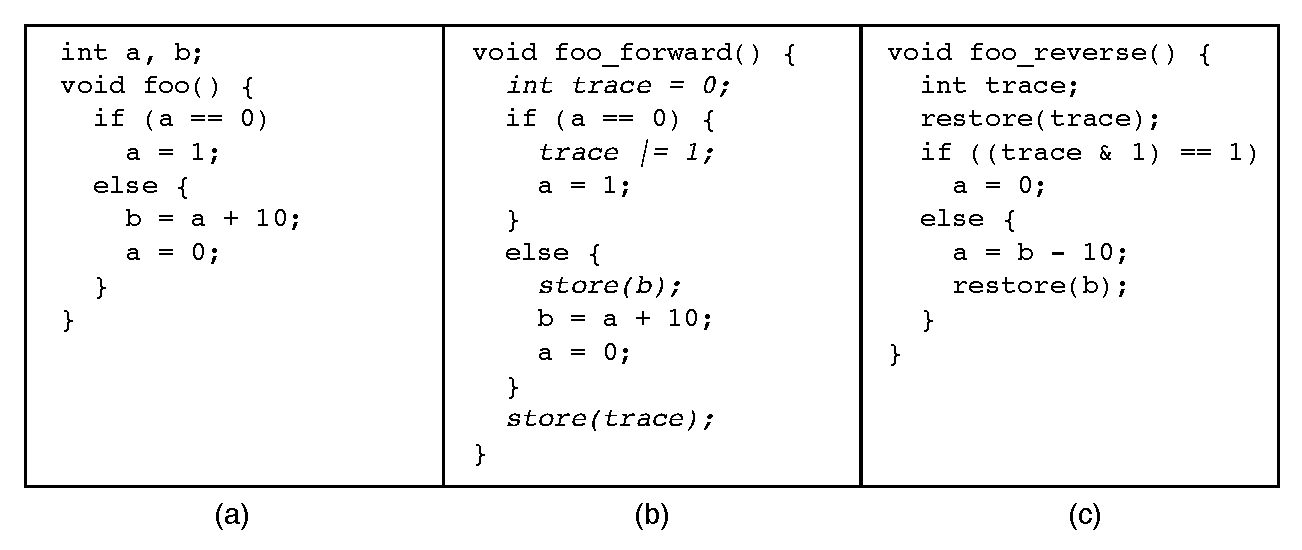
\includegraphics[width=400pt]{figures1/CodeExample.pdf}
\caption{(a) The original event $\quad$ (b) The forward event$\quad$ (c) The reverse event}
\label{fig:code_example}
\end{figure}


\section{Handling loop-free programs}


\subsection{Problem setup}
Let the set of \emph{target variables} be $S=\{s_1\dots s_n\}$ with \emph{initial values} $V=\{v_1 \dots v_n\}$, where $v_i$ is the initial value of $s_i$. These variables are modified by a \emph{target function}\footnote{The function here is a C/C++ function, not a function in mathematics.} $M$, producing $V' =\{v_1' \dots v_n'\}$, the \emph{final values} of the target variables. Our goal is generating two new functions, the \emph{forward function} $M^S_{fwd}$ and the \emph{reverse function} $M^S_{rvs}$, so that $M^S_{fwd}$ transfers $V$ to $V'$, and $M^S_{rvs}$ transfers $V'$ to $V$. We define \emph{available values} as values which are ready to use at the beginning of $M^S_{rvs}$. For example, values in $V'$ and constants are available values. We also call values in $V$ \emph{target values} which are values we want to restore from $M^S_{rvs}$.


Note that $M$ and $M^S_{fwd}$ have the same input and output, but $M^S_{fwd}$ is instrumented to store control flow information and values that are later used in $M^S_{rvs}$. 
This introduces two kinds of cost that must be considered when generating the forward-reverse pair $\{M^S_{fwd}, M^S_{rvs}\}$ : 
extra memory usage and run-time overhead.  


\subsection{Framework overview}

We will first treat the inversion of loop-free code with only scalar data types, without aliasing.
When such code is converted to static single assignment (SSA) form \cite{Cytron1991}, each versioned variable is only defined once and thus there is a one-to-one correspondence between each SSA variable and a single value that it holds.
We will also take advantage of the fact that loop-free code has a finite number of paths.
Loops will be discussed in the next section, and non-scalar data types and aliasing will not be handled in this paper.

Given a cost measurement, for each path in the target function there should exist a best strategy to restore target values. 
Strategies usually vary among different paths. 
Therefore, the reversed function we produce should include the best strategy for each path; each path in the original function should have a corresponding path in the reverse function. 

\begin{figure}
\centering
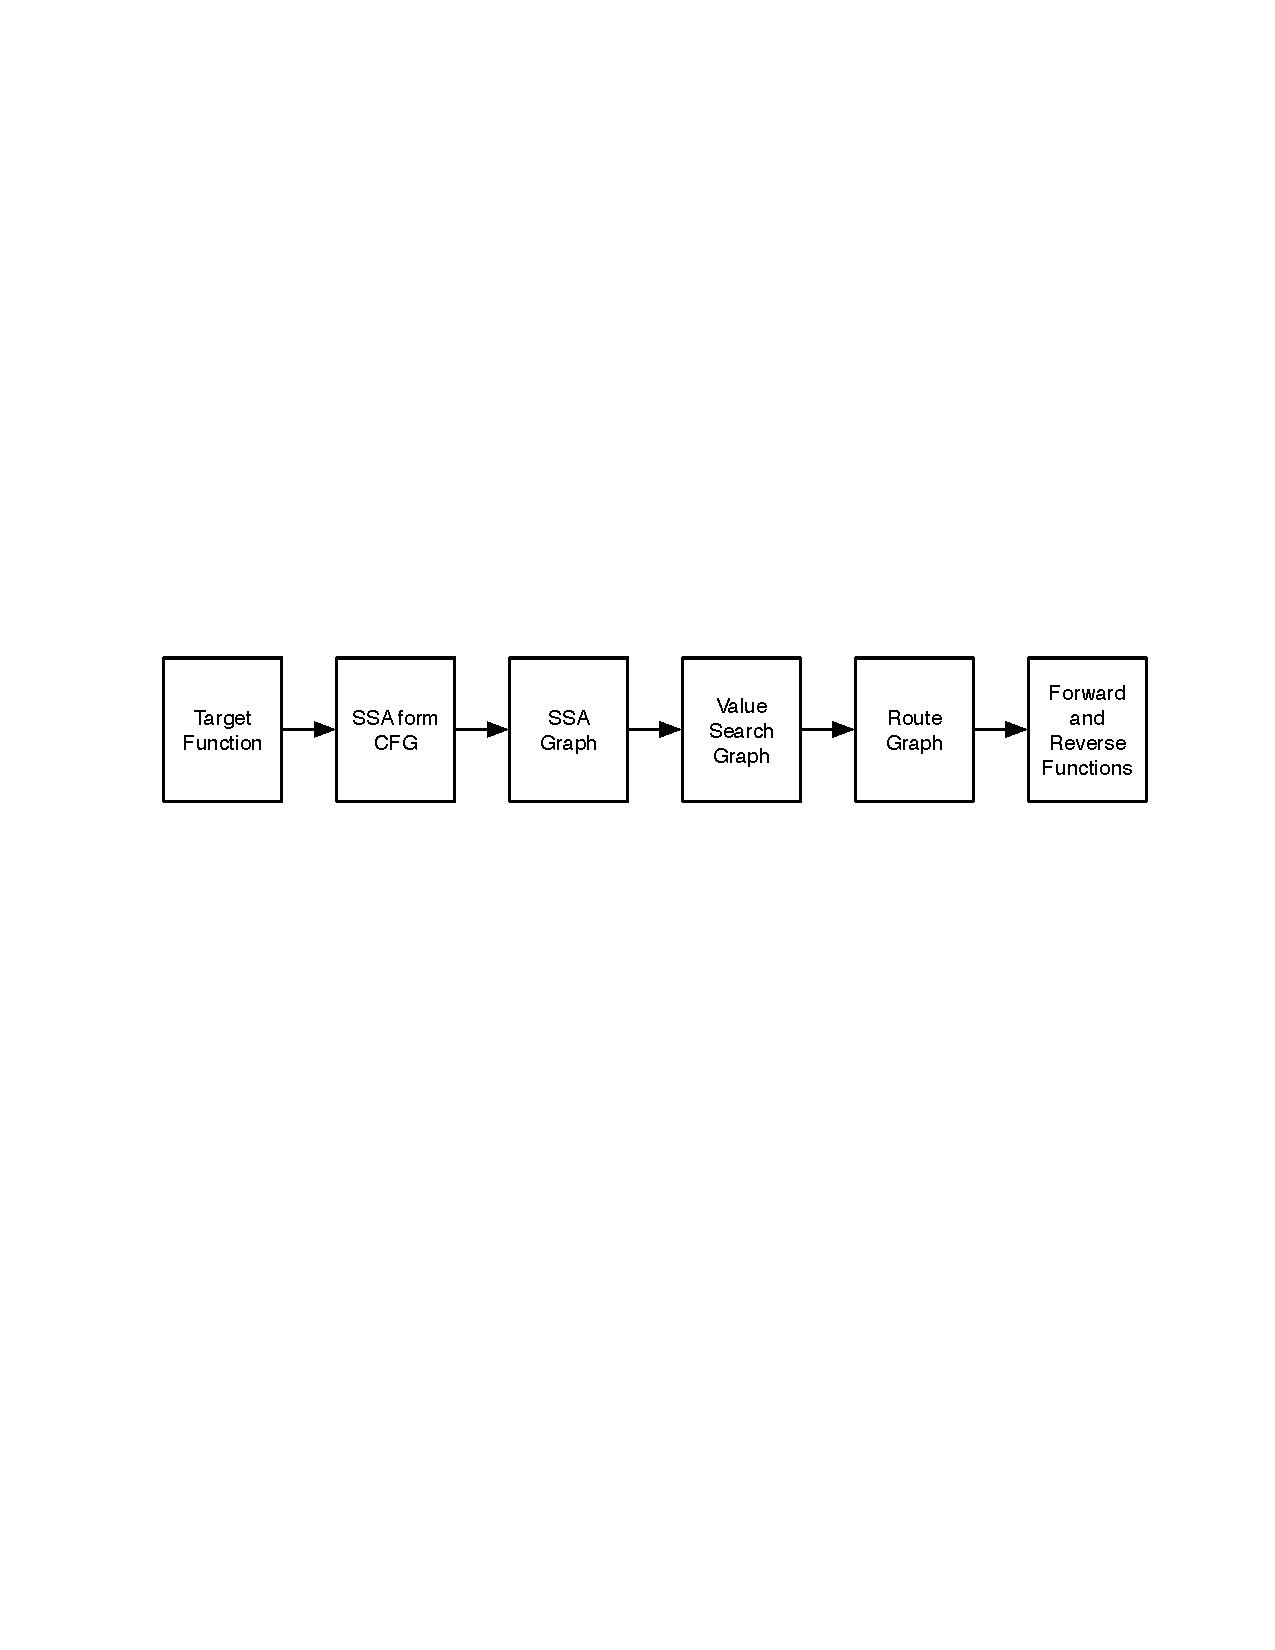
\includegraphics[width=400pt]{figures1/Framework.pdf}
\caption{Overall framework of the inversion algorithm}
\label{fig:framework}
\end{figure}

To restore target values, we will build a graph which shows equality relationships between values. 
We call this graph the \emph{value search graph}, and it is built based on an SSA graph \cite{Alpern1988,Cooper2001}. 
Then a search is performed on the value search graph to recursively find ways to recover the set of target values given the set of available values. 
If there is more that one way to restore a value, we choose the one with the smallest cost. 
The search result is a subgraph of the value search graph which we call a \emph{route graph}. 
For any path, a route graph shows a specific way to recover each target value from available values. 
Finally, the forward and reverse functions are built from a route graph. 
Figure \ref{fig:framework} illustrates this process.


\subsection{The value search graph (VSG)}
We first build an SSA graph for the target function.
An SSA graph \cite{Alpern1988,Cooper2001}, built based on SSA form, consists of vertices representing operators, function symbols, or $\phi$ functions, and directed edges connecting uses to definitions of values. It shows data dependencies between different variables. 
The full algorithm for building an SSA graph is presented in \cite{Muchnick}. 
Figure \ref{fig:VSG}(a)(b) show the SSA-transformed CFG and its SSA graph for the function in Figure \ref{fig:code_example}(a). In this example, \texttt{a} and \texttt{b} are two target variables with initial values \texttt{a$_0$} and \texttt{b$_0$}, and final values \texttt{a$_3$} and \texttt{b$_2$}.

\begin{figure}
\centering
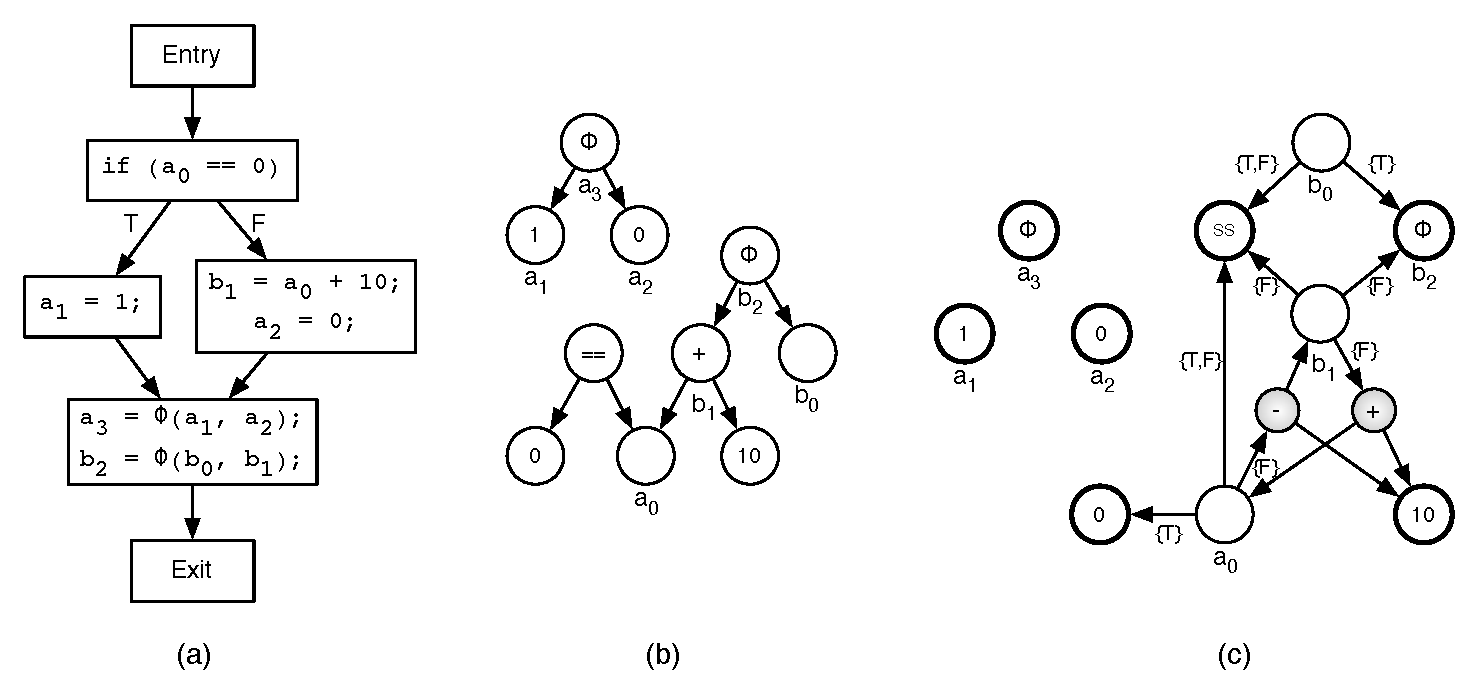
\includegraphics[width=400pt]{figures1/CFG.pdf}
\caption{(a) The SSA-transformed CFG of the function in Figure \ref{fig:code_example}(a)$\quad\quad$ (b) The corresponding SSA graph $\quad\quad$ (c) The corresponding value search graph. Nodes with bold outlines are available nodes; outgoing edges for these nodes are omitted because available nodes need not be recovered. `SS' is the special state saving node. Edges are annotated with their CFG path set.}
\label{fig:VSG}
\end{figure}




A \emph{value search graph} enables efficient recovery of values by explicitly representing equality relationships between values. 
Unlike an SSA graph, operation nodes are separated from value nodes in the value search graph, since their treatment is different for recovering values.
An edge connecting two value nodes $u$ and $v$ implies that $u$ and $v$ have the same value. 
%However, the equality of two values may only be true for certain CFG paths; hence each edge in a VSG is annotated with the set of CFG paths to which it applies.
An edge from value node $u$ to an operation node $op$ means that  $u$ is equal to the result of evaluating $op$ with its operands. 
To recover the value associated with node $v$, we can recursively search the graph starting at $v$.  

We attach a set of CFG paths to each edge in a value search graph, meaning the edge is applicable only if one of the CFG paths in that set is selected in the original function.
For operation nodes in the SSA graph, let the set of paths attached to each outgoing edge be the CFG paths for which the corresponding operation is executed. 
Similarly, for $\phi$ nodes, each reaching-definition edge should be annotated with all CFG paths for which the corresponding reaching definition reaches the $\phi$ function. 
We will describe an implementation of the path set representation later.

During the execution of the forward function, once a variable is assigned with a new value, its previous value may be destroyed and cannot be retrieved. To guarantee that a search in the value search graph can always restore a value, we introduce special \emph{state saving edges}. 
The idea behind these edges is that each value may be recovered by storing it during the forward execution. 
Whenever a state saving edge appears in the search results, the forward function is instrumented to save the corresponding value. 
The path set associated with a state saving edge for a value node $v$ is the set of all paths that include $v$'s definition. All state saving edges point to a unique \emph{state saving node}. %since it is not necessary to create a state saving node for every state saving edge.

\begin{comment}
\begin{figure}
\center{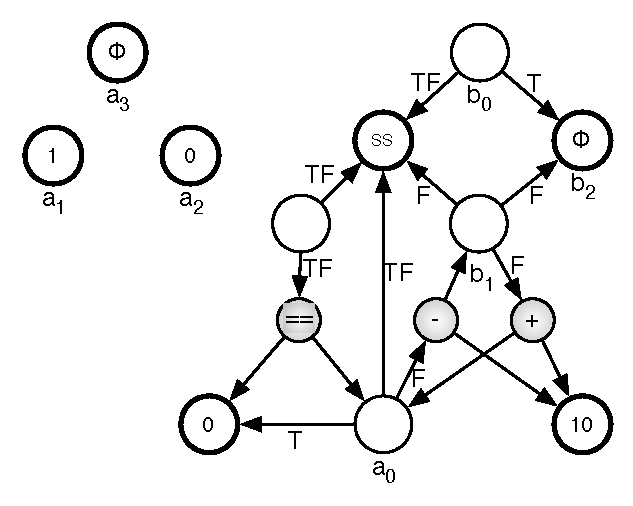
\includegraphics[width=160pt]{figures1/VSG.pdf}}
\caption{The value search graph for the function in Figure \ref{fig:code_example}(a). All available nodes are shown in bold. The label on edges from an operation node is only shown on the in-edge.}
\label{fig:VSG}
\end{figure}
\end{comment}

We apply the following rules to convert an SSA graph into a value search graph:
\begin{itemize}
	\item For simple assignment $v = w$, there is a directed edge from $v$ to $w$ in the SSA graph. 
	Since we can retrieve $w$ from $v$, add another directed edge from $w$ to $v$ with the same path set.

	\item A $\phi$ node in the SSA graph has several outgoing edges connecting all its possible definitions. 
	For each of those edges, add an opposite edge with the same path set. 
	
	\item For each operation node in the SSA graph, split it into an operation node and a value node, with an edge from the value node to the new operation node. 
	The new operation node takes over all outgoing edges, and the value node takes over all incoming edges. 
	
	\item If an equality operation (\texttt{==}) is used as a branching predicate and its outcome is true, we know that the two operands are equal.
	Therefore, we add edges from each operand to the other, with a path set for the edge equal to the path set of the \emph{true} CFG edge out of the branch. 
	We add the edges analogously for a not-equal operation (\texttt{!=}), but with the path set from the \emph{false} side of the branch.
	
	\item For every value that is not available, insert a state saving edge from the corresponding value node to the state saving node. 
\end{itemize}

\paragraph{Lossless operations} For certain operations, such as integer addition and exclusive-or, we can recover the value of an operand given the operation result and the other operand. For example, if $a=b+c$, we can recover $b$ given $a$ and $c$. For each such lossless operation, insert new operation nodes that connect its result to its operands, allowing the operands to be recovered from the result. The new nodes are added according to the following rules:
\begin{itemize}
	\item Negation (\texttt{a = -b}) and bitwise not (\texttt{a = \textasciitilde b}):$\;$ the new operations are  \texttt{b = -a} or \texttt{b = \textasciitilde a}, respectively.
	
	\item Increment (\texttt{++a}) and decrement (\texttt{--a}):$\;$ insert \texttt{--a} or \texttt{++a}, respectively.
	
	\item Integer addition (\texttt{a = b + c}) and subtraction:$\;$ for addition, the new operations are \texttt{b = a - c} and \texttt{c = a - b}; analogously for subtraction.
	
	\item Bitwise exclusive-or (\texttt{a = b \textasciicircum{ }c}):$\;$ insert \texttt{b = a \textasciicircum{ }c} and \texttt{c = a \textasciicircum{ }b}
\end{itemize}

\begin{comment}
\begin{figure}
\center{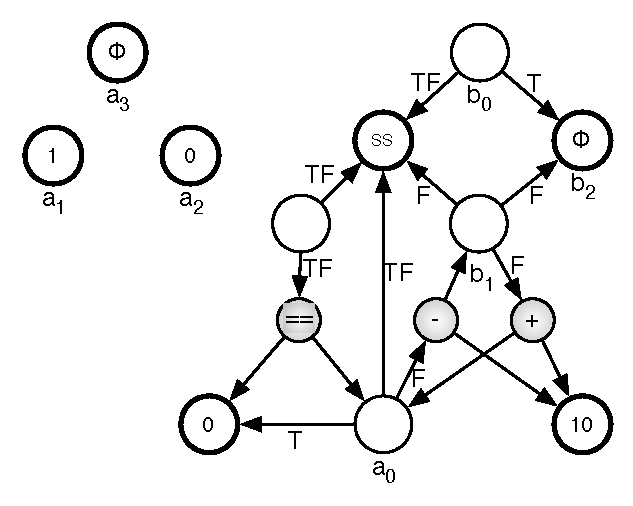
\includegraphics[width=160pt]{figures1/VSG.pdf}}
\caption{The value search graph for the function in Figure \ref{fig:code_example}(a). All available nodes are shown in bold. The label on edges from an operation node is only shown on the in-edge.}
\label{fig:VSG}
\end{figure}
\end{comment}

There are two special types of nodes in a value search graph: \emph{target nodes} are value nodes containing target values, and \emph{available nodes} are value nodes containing available values plus the state saving node.
As an optimization, we never create any outgoing edges for an available node. Figure \ref{fig:VSG}(c) shows the value search graph built for the code in Figure \ref{fig:code_example}(a). 
The available nodes are shown with a bold outline.
Since the function only has two paths, we use labels `T' and `F' to represent the CFG paths passing through the true and false body in the target function, respectively. 
The `--' operation node connecting $a_0$ to $b_1$ and the constant value `10' is generated from the `+' operation. 
The edge from $a_0$ to `0' for the path `T' is added based on the fact that $a_0 = 0$ on that path.
The `SS' node in the graph is the state saving node, and all unavailable nodes are connected to it. 
From the value search graph, we can find two valid ways to restore $b_0$ for the path `T': $b_0$ to SS node and $b_0$ to $b_2$. 
Obviously the second one is better since it avoids a state saving operation, and this better selection will be produced from the search algorithm described later.


\subsection{The route graph (RG)}
\label{sec:route-graph}

A \emph{route graph} is a subgraph of a value search graph connecting all target nodes to available nodes. Each route graph represents one way to restore the target values, and there may exist many valid route graphs for the same set of target values.
Edges in the route graph may have different path sets than the corresponding edges in the value search graph. 
For each edge $e$ in a route graph, let $P(e)$ denote the set of CFG paths that the edge is annotated with.
The following properties guarantee that the route graph properly restores all target values:

\begin{enumerate}[I)]

\item Let $\mathcal{U}$ be the set of all CFG paths. Then, for each target node $t$, 
	$$\bigcup_{\mathit{out} \in \text{OutEdges}(t)}P(\mathit{out}) \quad = \quad \mathcal{U} $$ 
	\label{rg-property-1}

\item For each node $n$ that is neither a target node nor an available node,
	$$\bigcup_{\mathit{out} \in \text{OutEdges} (n)} P(out) = \bigcup_{\mathit{in} \in \text{InEdges} (n)}P( \mathit{in} )$$ 

\item For each value node $n$, given any two outgoing edges $n\to p$ and $n\to q$, $P(n\to p) \cap P(n\to q) = \emptyset$ 

\item If $e$ is a route graph edge and its corresponding edge in the value search graph is $e'$, then $P(e) \subseteq P(e')$
	\label{rg-property-4}

\item For each directed cycle with edges $e_1 \dots e_n$,  $\quad \bigcup_{i=1}^n{P(e_{i})} = \emptyset$
	\label{rg-property-5}

\end{enumerate}

Property I specifies that each target value is recovered for every CFG path. 
Property II means that each value is recovered exactly for the paths for which it is needed.
Property III requires that for each CFG path, there is at most one way to recover a value. 
Property IV requires that the set of CFG paths associated with an edge in the route graph is a subset of the CFG paths originally associated with that edge in the value search graph. Finally, property V forbids self-dependence: restoring a value cannot require that value. 

\begin{figure}[htb]
\center{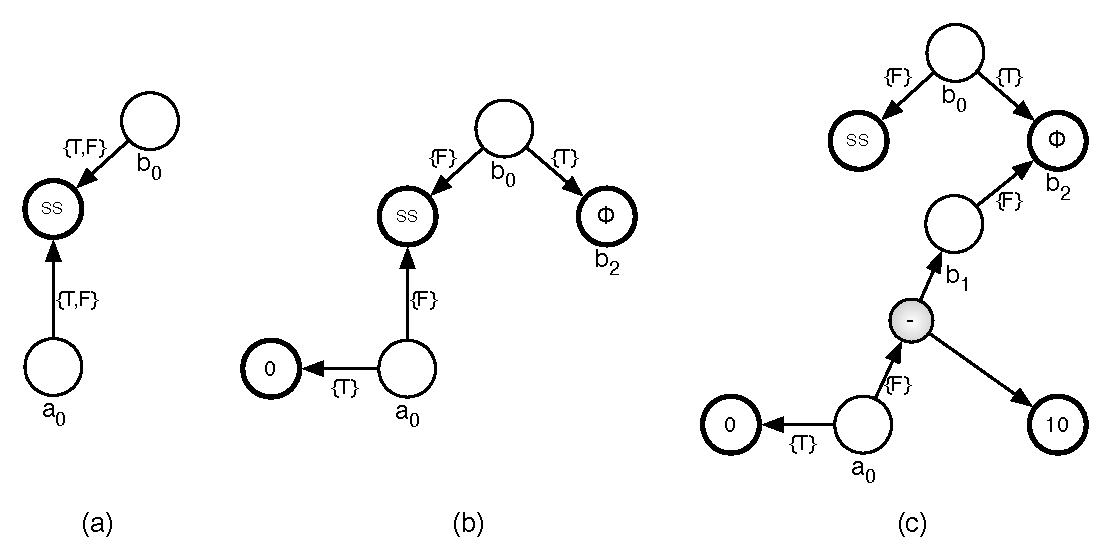
\includegraphics[width=400pt]{figures1/RG.pdf}}
\caption{Three different route graphs for the target values $\text{a}_{\text{0}}$ and $\text{b}_{\text{0}}$ given the the value search graph in Figure \ref{fig:VSG}(c). %While all three route graphs restore the target values, they have different costs.
}
\label{fig:RG}
\end{figure}

Figure \ref{fig:RG} shows three valid route graphs for the value search graph in Figure \ref{fig:VSG}. 
Route graph \ref{fig:RG}(a) only includes state saving edges. 
Route graph \ref{fig:RG}(b) takes advantage of the fact that for the `T' path the values of both \texttt{a$_0$} and \texttt{b$_0$} are known; it only uses staving for the `F' path. 
Route graph \ref{fig:RG}(c) improves upon route graph \ref{fig:RG}(b) by recomputing \texttt{a$_0$} as \texttt{b$_1$-10} for the CFG path `F'; state saving is only applied to \texttt{b$_0$} for path `F'.



\subsection{Searching the value search graph}

\subsubsection{Costs in route graphs}
As we have seen in Figure \ref{fig:RG}, there may be multiple valid route graphs that recover the target values, but with different overheads. 
In order to choose the route graph with the smallest overhead, we must define a cost metric.

Generally, there are two kinds of overhead in forward and reverse functions: execution speed and additional memory usage; we only consider the storage costs.
State saving contributes the most to the overhead memory usage and it also significantly affects the running time of both forward and reverse functions. 
Storing the path taken during forward execution is the other factor that contributes to memory usage; this overhead is bounded and is the same for all route graphs, so we exclude it from our cost estimate. 
With each state saving edge in the value search graph, we associate a cost equal to the size of the value that must be saved; other edges have cost 0.
%All other edges in the VSG have a small cost $\varepsilon$ associated with them, the technical reasons for which we will elucidate later. 
The cost of a route graph for a specific CFG path is the sum of the cost of those edges whose annotated path sets include that CFG path.

In Figure \ref{fig:RG}, suppose the cost to store and restore either \texttt{a} or \texttt{b} is $c$, the following table shows the cost of three route graphs for each CFG path.
% (here we ignore $\varepsilon$ just for clarity). 
Obviously the third route graph is the best one.

\begin{center}
\begin{tabular}{|c|c|c|c|}
%\begin{tabular}[c]{| c || m{1cm} | m{1cm} | m{1cm} |}
  \hline
  CFG path & route graph (a) & route graph (b) & route graph (c) \\
  \hline\hline
  T & $2c$ & $0$ & 0 \\
  \hline
  F & $2c$ & $2c$ & $c$ \\
  \hline
\end{tabular}
\end{center}

We have defined the cost of a single CFG path; however, a route graph may have different costs for different CFG paths.
When searching the value search graph, we would like to treat groups of CFG paths that share some edges in the route graph together, rather than performing a full search for each CFG path.
For this reason, the search algorithm partitions the CFG paths into disjoint sets of paths that have equal cost and we save the cost for each set of paths independently. 
In our search algorithm, we denote the costs of a route graph $r$ as $r.$costSet.
\[ r.\text{costSet} = \{ \langle P_{i}, c_{i} \rangle | P_{i}\text{ is a set of CFG paths and } c_{i} \text{ is the cost}\} \]
%\[P_{i} \cap P_{j} = \emptyset \quad \text{ if } i \neq j \]



\begin{algorithm}
\footnotesize
\label{algorithm:search}
\LinesNumbered
\DontPrintSemicolon

\SetKwData{NewCond}{newPaths}
\SetKwData{condition}{pathSet}
\SetKwData{cond}{paths}
\SetKwData{vertex}{target}
\SetKwData{edge}{edge}
\SetKwData{edges}{edges}
\SetKwData{edgeb}{e}
\SetKwData{target}{target}
\SetKwData{visited}{visited}
\SetKwData{subRoute}{newRoute}
\SetKwData{subGraph}{subGraph}
\SetKwData{route}{route}
\SetKwData{cost}{cost}
\SetKwData{eCopy}{eCopy}
\SetKwData{target}{target}
\SetKwData{subRoutes}{subRoutes}
\SetKwData{result}{resultRoute}
\SetKwData{costSet}{costSet}
\SetKwInOut{Input}{Initial input}

\SetKwFunction{OutEdges}{OutEdges}
\SetKwFunction{SearchSubRoute}{SearchSubRoute}
\SetKwFunction{SearchRoute}{SearchRoute}
\SetKwFunction{UpdateConditions}{ChooseMinimalCosts}

\Input{The search start point \vertex, with \cond $= \emptyset$, \visited $= \emptyset$}




\BlankLine
\SearchSubRoute{\vertex, \cond, \visited} \;
\Begin{
  \result $\leftarrow \emptyset$,  \subRoutes $\leftarrow \emptyset$ \;
  \If{\vertex is an operation node}{
      \ForEach{\edge $\in$ \OutEdges{\vertex}}{
          \lIf{\edge.\target $\in$ \visited}{\Return $\emptyset$\;}
          \subRoute $\leftarrow$ \SearchSubRoute{\edge.\target, \cond, \visited}\; 
          \lIf{\subRoute $= \emptyset$}{\Return $\emptyset$\;}
          add \edge and \subRoute to \result \;
      }
      \Return \result \;
  }
  \If{\vertex \mbox{is available}}{
      add \vertex to \result \;
      add $\langle \cond, 0 \rangle$ to \result.\costSet \;
      \Return \result \;
  }
  \ForEach{\edge $\in$ \OutEdges{\vertex}}{
    \lIf{\edge.\target $\in$ \visited}{continue}  
    \BlankLine
    \NewCond $\leftarrow$ \edge.\condition $\cap$ \cond\; 
    \lIf{\NewCond $=  \; \emptyset$}{continue} 
    \BlankLine

    \subRoute $\leftarrow$ \SearchSubRoute{\edge.\target, \NewCond, \visited$\cup \; \{\vertex\}$}\;
 
    add \edge with paths \NewCond to \subRoute\;
    \lForEach{$\langle \cond, \cost \rangle$ in $\subRoute.\costSet$}{
        \cost += \edge.\cost\;
    }
        \lForEach{\route in \subRoutes}{
    \UpdateConditions{\route, \subRoute}\;
    }


      add \subRoute to \subRoutes \;

  }
  add \vertex to \result \;
  \ForEach{\route in \subRoutes}{
      \lIf{$\route.\condition \ne \emptyset$}{
          add \route to \result \;
      }
  }
  \Return \result \;
}

\SetKwData{routea}{route1}
\SetKwData{condition}{pathSet}
\SetKwData{routeb}{route2}
\SetKwData{edge}{edge}
\SetKwData{graph}{routeGraph}
\SetKwData{conda}{paths1}
\SetKwData{condb}{paths2}
\SetKwData{costa}{cost1}
\SetKwData{costb}{cost2}
\SetKwData{paths}{paths}
\SetKwData{cost}{cost}

\BlankLine
\BlankLine
\UpdateConditions{\routea, \routeb} \;
\Begin{
    \lIf{\routea.\condition $\cap$ \routeb.\condition  $ = \emptyset$}{
        return\;
    }
    \ForEach{$\langle \conda, \costa \rangle$ in \routea.\costSet}{
        \ForEach{$\langle \condb, \costb \rangle$ in \routeb.\costSet}{
            \lIf{\conda $\cap$ \condb $= \emptyset$}{
                continue\;
            }
            \If{\costa $>$ \costb} {$\conda \leftarrow \conda - \condb $\;
            Remove (\conda $\cap$ \condb) from all edges of \routea \;}
            \Else{$\condb \leftarrow \condb - \conda $\;
            Remove (\conda $\cap$ \condb) from all edges of \routeb \;}
        }
    }
    \routea.\condition $ = \bigcup_{\langle \paths, \cost \rangle \in \routea.\costSet} \paths $ \;
    \routeb.\condition $ = \bigcup_{\langle \paths, \cost \rangle \in \routeb.\costSet} \paths $
}

\caption{Searching for a route graph in a value search graph}

\end{algorithm}

\subsubsection{Search algorithm}
Our search algorithm should aim to find a route graph that has the minimum cost for each path. 
Theoretically, however, searching for a minimal route graph is an NP-complete problem. 
To make the problem tractable, we apply the heuristic of finding a route graph for each target value individually; the individual route graphs are then merged into a route graph that restores all the target values. 
Similarly, in order to recover the value of a binary operation node, we recover each of the two operands independently and then combine the results. 

The pseudocode for our heuristic search algorithm is presented in Algorithm \ref{algorithm:search}. 
The {\tt SearchSubRoute} function returns a route graph given a target node, the paths for which that node must be restored, and the set of value nodes visited so far.
The algorithm explores all ways to recover the current node by calling itself recursively on all the nodes that are directly reachable from the current node; available nodes are the base case.
Lines 5--10 handle recovering the values of operation nodes. 
In order to recover the value of an operation node, each of its operands must be recovered.
Lines 11--14 return a trivial route graph for available nodes, with a cost of 0. 
The remaining body of the algorithm (lines 15--27) handles recovering a value node that is not available.
Each of the out-edges of the target node may be used to recover its value for the CFG paths associated with that edge; these edges are explored in the {\tt for}-loop in lines 15--23.
The variable {\tt newPaths} on line 17 represents the set of paths that we are both interested in and are associated with the current edge. 
In line 19, we recursively find a route graph that recovers the target value by recovering the target of the current outgoing edge.
Lines 21--22 update the cost sets of the new route graph; if it provides a lower cost for some CFG path than the solutions found so far, the partial results are modified so that each CFG path is restored with the cheapest route graph.
Finally, the route graph from line 19 is added to the list of partial results (line 23). 
After all out-edges of the target node have been explored, the partial results are merged into a single route graph and returned (lines 24--27).
Note that it is unnecessary to check whether the target node has been successfully recovered, since the state saving edge always provides a valid route graph for the node. 
Figure \ref{fig:RG}(c) shows the route graph produced by the algorithm when searching the value search graph from Figure \ref{fig:VSG}(c).

The search algorithm enforces properties \ref{rg-property-1}--\ref{rg-property-4} from section \ref{sec:route-graph} during its execution.
To make sure that the search result does not contain cycles (property \ref{rg-property-5}), we record which value nodes are already in the route using a set \texttt{visited} in Algorithm \ref{algorithm:search}. 
This alone is not sufficient to guarantee that the result is acyclic, for there may be two different paths with identical cost to recover a single value node. 
If one way is chosen to recover a value node $v$ during path of the search, and then later $v$ is recovered differently for the same CFG path, a cycle may form.
To prevent this situation from occurring, we always traverse out-edges in the same order of line 19 of Algorithm \ref{algorithm:search}; the first route graph with the smallest cost is chosen. In addition, two paths coming from two different value nodes may also form a cycle when all costs on edges of the cycle are 0. We eliminate this possibility by replacing 0 by a small cost $\varepsilon$.
% Do we really need to have epsilon for correctness? It seems that the above condition is sufficient to guarantee correctness

\begin{comment}
\paragraph{Extensions} Adding constraints during the search could produce different inversion strategies. 
For example, putting only state saving edges to the route graph will produce the same result as checkpointing.
Including state saving edges and phi edges (edges incident to a phi node) results in the incremental state saving, where a variable is saved only for the paths for which it is modified. 
\end{comment}

\subsection{Instrumentation \& Code generation}

\subsubsection{Representing CFG path sets}

Our search algorithm relies on efficiently computing intersection, union, and complement of CFG path sets, as well as testing whether the set of paths is empty; for this reason we suggest implementing the set representations as bit vectors. 
Ball and Larus \cite{Ball1996} present an path profiling method in which each path is given a number from 0 to $m-1$, where $m$ is the count of the CFG paths. 
We use their algorithm to number each path, and for each path we associate exactly one bit in the bit vector used to represent a path set.
%Algorithm \ref{algorithm:findPaths} illustrates how to use depth-first search on the CFG to find the set of paths that correspond to each CFG edge; the search is initially invoked with \texttt{FindCfgPaths(Entry, 0)}.

\begin{comment}

\begin{algorithm}
\label{algorithm:findPaths}
\DontPrintSemicolon
\caption{Finding the set of paths passing through each CFG edge}



\SetKwFunction{findCfgPaths}{FindCfgPaths}
\SetKwFunction{OutEdges}{OutEdges}

\SetKwData{node}{node}
\SetKwData{edge}{edge}
\SetKwData{target}{target}
\SetKwData{pathIndex}{pathIndex}
\SetKwData{exitNode}{\textbf{Exit}}
\SetKwData{pathsHere}{pathsFound}
\SetKwData{pCount}{count}

\BlankLine
\findCfgPaths{\node, \pathIndex} \;
\Begin{
	\lIf{\node == \exitNode}
	{
		\Return 1 \;
	}
	\pathsHere $\leftarrow$ 0 \;

	\ForEach{\edge $\in$ \OutEdges{\node}}
	{
		\pCount $\leftarrow$ \findCfgPaths{\edge.\target, \pathIndex} \;
		Add paths \pathIndex through (\pathIndex + $\pCount - 1$) to \edge \;
		\pathsHere $\leftarrow$ \pathsHere + \pCount \;
		\pathIndex $\leftarrow$ \pathIndex + \pCount \;
	}
	\Return{\pathsHere} \;
}

\end{algorithm}

\end{comment}

\subsubsection{Recording CFG paths}
\label{sec:encoding-paths}
\begin{comment}
We can encode a path with a path number as above, and checking if a path set represented by a bit vector contains a path is also fast. However, the length of a bit vector equals the number of CFG paths, which can be large. Further, we will see later that each branch in the reverse function is translated from the path set on a route graph edge. If there are $m$ CFG paths in the target function, and $n$ distinct path sets used to generate the predicates in the reverse function, then we need $m\times n$ bits of static memory in the reverse function! %Another problem comes that we may also need the condition  in the forward method for the state saving statement. 
Our solution is using another method to encode CFG paths. We will see that a path set can be transformed to a set of new representations, from which we can build more efficient predicates in the reverse function.
\end{comment}

We need to store path information in a way that allows us to efficiently record the CFG path taken (for forward execution), and to efficiently check if the path matches a given set of CFG paths attached to a route graph edge (for reverse execution). 
However, if we encode each path using its path number, then examining whether a path is a member of a set is inefficient.
% (we don't want each path set represented by a bit vector to appear in the reverse code, which may take too much memory). 
Instead we  %employ another approach to encoding paths, and 
use a bit vector to record the CFG path, in which each bit represents the outcome of a branching statement. 
%We will see later that this new path encoding will result in quite efficient comparisons in the reverse execution.
Since this method is similar to \emph{bit tracing}\cite{Ball1994}, we call this bit vector a \emph{trace}.
Note that two branches may share the same bit if they cannot appear in the same path. Thus, the number of bits required to store the path taken is equal to the largest number of branches that appear on a single CFG path.
Algorithm \ref{algorithm:conditions} calculates bit-vector position for each branch node accordingly.

\begin{algorithm}
\label{algorithm:conditions}
\DontPrintSemicolon

\SetKwData{vertex}{u}
\SetKwData{vertexa}{v}
\SetKwData{vertexb}{w}
\SetKwData{mask}{mask}
\SetKwFunction{bitPosition}{position}
\SetKwFunction{maxVal}{max}

\BlankLine
\BlankLine
    \ForEach{CFG node \vertex in reverse topological order}{
        \uIf{\vertex is a leaf node}{
            \bitPosition{\vertex} $\leftarrow$ -1 \;
        }
            \uElseIf{\vertex is a branch node}{
                \tcc{$\vertex\to\vertexa$ and $\vertex\to\vertexb$ are its two out-going edges} 
                \bitPosition{\vertex} $\leftarrow$ \maxVal{\bitPosition{\vertexa}, \bitPosition{\vertexb}} + 1\;
            }
            \Else{ 
                \tcc{$\vertex\to\vertexa$ is its out-going edge} 
                \bitPosition{\vertex} $\leftarrow$ \bitPosition{\vertexa} \;
            }         
    }

\caption{Generating the bit position for each branch node.}
\end{algorithm}

In the forward function, we use an integer as the bit vector to record all predicate results\footnote{Potentially we could omit recording predicates that do not affect the reverse function.}. 
Let \texttt{trace} be the variable recording a trace, initialized to zero; then the true edge of each branch node $v$ is instrumented with the statement \footnote{We use several operators in C/C++ syntax here and below, which includes bitwise OR operator \texttt{|}, bitwise AND operator \texttt{\&}, bitwise left shift operator  \texttt{<<}, equal to operator \texttt{==}, and logical OR operator \texttt{||} .}
$$ \texttt{trace = trace  | (1 << $\mathit{position(v)}$)}; $$ 
where $\mathit{position(v)}$ is calculated by Algorithm \ref{algorithm:conditions}. 
The variable \texttt{trace} is stored at the end of the forward function and restored at the beginning of the reverse function. 
Note that we can further optimize the instrumentation by moving a trace updating operations downward through the CFG and merging them.
%The Ball and Larus maximal spanning tree method for calculating edges to instrument is also applicable \cite{Ball1996}. 



In the reverse function, we must test if \texttt{trace} matches the path sets that appear on route graph edges. We start with transforming each path in the set into a trace (the trace for each path can be computed by the same means as recording a trace in the forward function).
Then, checking if a path set contains a path represented by \texttt{trace} is done by comparing it to each trace. 
Suppose a path set containing two paths is transformed into two traces \texttt{01101} and \texttt{01001}. Instead of comparing \texttt{trace} to each of them as:
$$ \texttt{if (trace == 01101 || trace == 01001)} $$ 
we can simplify this predicate by using a mask \texttt{11011} on \texttt{trace}:
$$ \texttt{if ((trace \& 11011) == 01001)} $$ 

The combined trace for \texttt{01101} and \texttt{01001} is \texttt{01$\times$01}, where $\times$ denotes that the bit does not matter. 
Given a set of traces, we can combine pairs repeatedly to reduce the size of the set.
This greatly reduces the complexity of the branching statements in the reverse code. 
\begin{comment}

Each CFG path is induced by a sequence of branches that must be either true or false; we can build the corresponding mask by setting 0 or 1 in the position corresponding to each branch. 
Some elements of the mask representing a CFG path may be $\times$, which signifies that the outcome of the corresponding branch does not affect whether the path is taken or not. 
Algorithm \ref{algorithm:computeMasks} computes the path mask associated with each CFG path; it is initially invoked as \texttt{ComputePathMasks(Entry, 0, $\times$$\times$$\dots$$\times$$\times$)}. 
Note that the indices computed for each path by Algorithm \ref{algorithm:computeMasks} match those computed by Algorithm \ref{algorithm:findPaths}; in fact, these two algorithms can be merged into one. 


\begin{algorithm}
\label{algorithm:computeMasks}
\DontPrintSemicolon
\caption{Finding mask corresponding to each CFG path}

\SetKwFunction{computePathMasks}{ComputePathMasks}
\SetKwFunction{OutEdges}{OutEdges}

\SetKwData{node}{node}
\SetKwData{edge}{edge}
\SetKwData{target}{target}
\SetKwData{pathIndex}{pathIndex}
\SetKwArray{currentMask}{currentMask}
\SetKwData{exitNode}{\textbf{Exit}}
\SetKwData{pathsHere}{pathsFound}
\SetKwData{pCount}{count}
\SetKwFunction{bitPosition}{position}
\SetKwData{edgeLabel}{label}

\BlankLine
\computePathMasks{\node, \pathIndex, \currentMask} \;
\Begin{
	\If{\node = \exitNode}
	{
		\currentMask is the mask for the path \pathIndex \;
		\Return 1
	}
	\pathsHere $\leftarrow$ 0 \;

	\ForEach{\edge $\in$ \OutEdges{\node}}
	{
		\If{\edge is labeled} 
		{
			\currentMask{\bitPosition{\node}} $\leftarrow$ 
			$\begin{cases} 0 \text{ if } \edge.\edgeLabel = F \\ 1 \text{ if } \edge.\edgeLabel = T \end{cases}$
		}
		\pCount $\leftarrow$ \computePathMasks{\edge.\target, \pathIndex, \currentMask} \;
		\pathsHere $\leftarrow$ \pathsHere + \pCount \;
		\pathIndex $\leftarrow$ \pathIndex + \pCount \;
	}
	\Return{\pathsHere} \;
}

\end{algorithm}

In order to test the recorded path against a set of CFG paths, we may test the mask of the path against each of the masks in the set. 
For example, we can test for the mask 00$\times$10 with \texttt{((cfgmask \& 11011) == 00010)}.
To make these checks more efficient, however, we may merge multiple CFG paths into a single mask.
For example, if the masks for two paths are $0011$ and $0111$, we can test for either path with the mask 0$\times$11. 

\end{comment}


Algorithm \ref{algorithm:mergeMasks} starts out with all traces corresponding to a set of CFG paths and merges them into a minimal set of traces that can be used to test membership in the set. 
The intuition behind Algorithm \ref{algorithm:mergeMasks} is that if the traces are sorted so that bit $i$ is the least significant bit, the traces that are identical to each other except for bit $i$ will be adjacent. 
However, if we are careful we don't have to pay the full sorting cost for each bit $i$. 
If the traces are sorted when their bits are considered in the order $b_{1} b_{2} \dots b_{i - 1} \quad b_{k} b_{k - 1} \dots b_{i} $ and we want to sort them according to the bit order $b_{1} b_{2} \dots b_{i - 2} \quad b_{k} b_{k - 1} \dots b_{i - 1} $, we need only sort each sequence of the trace for which bits 1 through $(i-2)$ are identical. 
For each such sequence, there are at most three sorted subsequences, indexed by bit $b_{i-1}$; these can be merged in linear time (similarly to mergesort).
If we use a linear-time sort, such as radix sort, for the first iteration, the overall runtime of Algorithm \ref{algorithm:mergeMasks} is $O(k n)$, where $n$ is the size of the path set.


\begin{algorithm}
\label{algorithm:mergeMasks}
\DontPrintSemicolon
\caption{Merging a set of path traces}

\SetKwFunction{mergePathMasks}{MergePathTraces}

\SetKwArray{masks}{traces}
\SetKwData{bitSize}{k}
\SetKwData{index}{i}
\SetKwData{maskIndex}{j}

\SetKw{KwDownTo}{down to}

\SetKwFunction{length}{Length}

\mergePathMasks{\masks} \;
\Begin{
	\tcc{Each trace has \bitSize "bits", and each bit is 0, 1, or $\times$}
	\tcc{Bits are numbered ascendingly; e.g. $m = b_{1} b_{2} \dots b_{k}$}

	\For{\index $\leftarrow$ \bitSize \KwDownTo $1$}
	{
		\tcc{Note: for \index = k, the bit ordering is $m = b_{1} b_{2} \dots b_{k}$}
		Sort \masks, where trace bits are ordered $b_{1} b_{2} \dots b_{i - 1} \quad b_{k} b_{k - 1} \dots b_{i} $ \;
		
		\For{\maskIndex $\leftarrow$ 2 \KwTo \length{\masks}}
		{
			\If{ \masks{\maskIndex$-\;1$} and \masks{\maskIndex} match except for bit \index}
			{
				set bit \index to $\times$ for  \masks{\maskIndex$-\;1$} \;
				delete \masks{\maskIndex}
			}
		}
	}
	

	
}

\end{algorithm}

After the merge, if we have $n$ traces $t_1,...,t_n$ for a path set, the resulting predicate would be:
$$\texttt{if ((trace \& $mask_1$) == $obj_i$ || ... || (trace \& $mask_n$) == $obj_n)$}$$
For each trace $t_i$, $mask_i$ is obtained by setting all bits which are $\times$ in $t_i$ to 0 and others to 1, and $obj_i$ equals $mask_i$ \texttt{\&} $t_i$.



\subsubsection{Inserting state saving statements}
\label{sec:state-saving}
The other instrumentation in the forward function are state saving statements, which are inserted according to the state saving edges in the route graph. 
For each state saving edge in the route graph, suppose the variable to store is $var$ and the path set on this edge is $P$. 
Our task is finding one or several locations to store $var$ according to the path set $P$, ensuring that $var$ is only saved once for each CFG path in $P$. 

To find such locations, we first compute the corresponding path traces $T$ of $P$ from Algorithm \ref{algorithm:mergeMasks}. 
For each trace in $T$, we traverse the CFG from the entry. 
When we reach a branch node, check the corresponding bit in the trace: fall through the true edge if the bit is 1, false edge if the bit is 0. 
If the bit is $\times$, the traversal forks and that bit is assigned to 0 and 1 respectively forming two new traces; and for each concretized trace the descent continues. 
The descent stops immediately when all bits which are not checked in the trace are $\times$. 
After this process, we obtain one or more locations where the descent has stopped. 
%This is not clear. It's better to leave it out than to have it be confusing
%If the tracings from two traces stop at the same location, we then combine them again (since they may be forked from one trace previously). 
%In each maximal basic block in which each location resides, 
In each location we find a point where the definition of $var$ is reachable and a state saving statement is inserted there. 
However, it is possible that the path set containing the paths passing through this location is larger than the one on which the state saving is needed. 
In this case, we guard the state saving statement with a branch whose predicate corresponds to the trace at this location.



\subsubsection{Building a CFG for the reverse function}
We build the CFG for the reverse function from a route graph; the reverse CFG is acyclic and each path in it must obey the data dependencies represented in the route graph.
Each outgoing edge from a value node in the route graph will be translated to a statement in the reverse function. 

There could be a large number of correct reverse CFGs for a route graph, resulting in different control flows and different numbers of branches. 
%Without the runtime information such as profiling data, it is difficult to determine with one is the best with respect to the performance. 
We choose to build a structured CFG to simplify the translation to source code. 
We also attempt to minimize the number of predicates in the CFG. 

There are three kinds of statements that can be generated from a route graph:
\begin{itemize}
	\item An operator node with its operands and result induces an operation statement,  such as \texttt{a = b + c}.
	\item An edge with value nodes as both ends induces an assignment statement.
	\item An edge pointing to the SS node induces an value restoration statement.
\end{itemize}

%For the purposes of code generation, we shall refer to an operation node together with its incoming and outgoing edges as an operation (hyper)edge, which is a special edge with one source and one or more targets.
%With this convention, each statement corresponds to one ``edge'' in the route graph.

The statements generated from route graph edges retain the path sets attached to the corresponding edges.
We build basic blocks of statements that all share the same path sets, and insert branches so that each basic block is executed when the corresponding path is taken in the forward function. 
While enforcing the path set constraints ensures correct control flow, producing correct data flows depends on the order in which statements are inserted in the CFG.
Note that a route graph corresponds to explicit data dependencies, and for each CFG path in the forward function it is acyclic due to property \ref{rg-property-5} from section \ref{sec:route-graph}. 
Hence, if we order statements in the reverse topological order of the route graph edges, dataflow dependencies are correctly maintained.

\begin{algorithm}
\footnotesize
\label{algorithm:reverse-cfg}
\LinesNumbered
\DontPrintSemicolon
\caption{Generating a CFG for the reverse function from a route graph.}


\SetKwData{bb}{b}
\SetKwData{bone}{b1}
\SetKwData{btwo}{b2}
\SetKwData{stmts}{pendingStmts}
\SetKwData{bbs}{openBlocks}
\SetKwData{s}{s}
\SetKwData{cond}{pathSet}
\SetKwData{cp}{pathSetPairs}
\SetKwData{edge}{edge}
\SetKwData{valNode}{valNode}
\SetKwData{RG}{routeGraph}
\SetKwData{CFG}{cfg}
\SetKwData{source}{source}
\SetKwData{availNode}{availNode}
\SetKwFunction{GenerateReverseCFG}{GenerateReverseCFG}
\SetKwFunction{GetStatements}{BuildReadyStatements}
\SetKwFunction{InEdges}{InEdges}

\SetKwFunction{BuildBB}{BuildBasicBlock}
\SetKwData{entry}{entry}

\BlankLine
\GenerateReverseCFG{\RG}\\
\Begin
{
	\CFG $\leftarrow \emptyset$, \stmts $\leftarrow \emptyset$, \bbs $\leftarrow \emptyset$, \cp $\leftarrow \emptyset$\; 
	\lForEach{\valNode in \RG}
	{
		\valNode.\cond $\leftarrow \emptyset$\;
	}
	\ForEach {available node \availNode in \RG}
	{
		\GetStatements{\availNode, $\mathcal{U}$, \stmts} \;
	}
	\CFG.\entry $\leftarrow$ \BuildBB{$\mathcal{U}$} \;
	%Create a new basic block with path set $\mathcal{U}$ as the entry of the CFG and add it to \CFG and \bbs\;
    
	\While{$\stmts \neq \emptyset$}
	{
		\uIf{$\exists \s \in \stmts, \bb \in \bbs$, and $\s.\cond = \bb.\cond$}
		{
			Append \s to \bb\;
			\valNode $\leftarrow$ the source node of the edge that generated \s \;
			 \GetStatements{\valNode, \s.\cond, \stmts}\;
 		}
		\uElseIf{$\exists \s \in \stmts, \bb \in \bbs$, and \s.\cond $\subset$ \bb.\cond}
		{
			Append to \bb a branch, with the predicate generated from \s.\cond\;
			\bone $\leftarrow$ \BuildBB{\s.\cond} \;
			Append \s to \bone\;
			\btwo $\leftarrow$ \BuildBB{$\bb.\cond - \s.\cond$} \;
			%Create two new basic blocks $\bone$ and $\btwo$ with path set \s.\cond and $\bb.\cond - \s.\cond$ respectively, and add them to \CFG and \bbs\;
			Insert into \CFG edges from \bb to \bone and \btwo with labels \textit{true} and \textit{false} \;
			Add $\langle \bone.\cond, \btwo.\cond \rangle$ to \cp\;
			\bbs $\leftarrow \; \bbs - \{ \bb \}$ \;
			%Remove  \bb from \bbs\;
			\valNode $\leftarrow$ the source node of the edge that generated \s \;
			\GetStatements{\valNode, \s.\cond, \stmts}\;
 		}
		\ElseIf{$\exists \bone, \btwo \in \bbs$, and $\langle \bone.\cond, \btwo.\cond \rangle \in \cp$}
		{
			\bb $\leftarrow$ \BuildBB{\bone.\cond $\cup$ \btwo.\cond} \;
			%Create basic block \bb, $\bb.\cond = \bone.\cond \cup \btwo.\cond$, and add \bb to \CFG and \bbs\;
			Insert into \CFG two edges, from \bone and \btwo to \bb\;
			\cp $\leftarrow \; \cp - \{ \langle \bone.\cond, \btwo.\cond \rangle \}$ \;
			%Remove $\langle \bone.\cond, \btwo.\cond \rangle$ from $\cp$\;
			\bbs $\leftarrow \; \bbs - \{ \bone, \btwo \}$ \;
			%Remove \bone and \btwo from \bbs\;
			\lIf{$|\bbs| = 1$}{break}
		}
	}
	\Return{\CFG}
}

\BlankLine

\SetKwData{availablePathSets}{nodeAvailablePaths}

\GetStatements{\valNode, \availablePathSets, \stmts}\\
\Begin
{
	\valNode.\cond $\leftarrow$ \valNode.\cond $\cup$ \availablePathSets \;
	\ForEach{\edge $\in$  \InEdges{\valNode}}
	{
		\If{\edge.\cond $\subseteq$ \valNode.\cond}
		{
			\uIf{\edge.\source is an operation node}
			{
				Set \edge to be a available for \edge.\source \;
				\If{all operands of \edge.\source are available}
				{
					Add to \stmts the statement for for \edge.\source, with path set \edge.\cond \;
				}
			}
		\Else
		{
			Add to \stmts the statement for \edge, with path set \edge.\cond \;
		}}
	}
}
\BlankLine

\BuildBB{\cond}
\Begin
{
	Build an empty basic block \bb and attach path sets \cond to it. \;
	\CFG $\leftarrow$ \CFG $\cup$ \{ \bb \}, $\quad$
	\bbs $\leftarrow$ \bbs $\cup$ \{ \bb \} \;
	\Return{ \bb } \;
}

\end{algorithm}

Algorithm \ref{algorithm:reverse-cfg} shows how to build a CFG for the reverse function. 
We keep a set of basic blocks, \texttt{openBlocks}, to which new statements can be appended.  
We also maintain a set of statements, \texttt{pendingStmts}, whose data dependencies have been satisfied, but which have not yet been inserted in the CFG.
Each basic block has an associated path set; these are the paths in the forward function for which the corresponding basic block in the reverse function should execute.
Similarly, each statement has a set of paths from the forward function. 
If there is a pending statement and an open basic block whose path sets match, we simply append the statement to the basic block.
When a statement is inserted into the CFG, the data dependencies of new statements may now be satisfied; we call the function \texttt{BuildReadyStatements} to generate the statements that are now valid for insertion. 
If there is no pending statement whose path set matches the path set of an open basic block, we must insert or join a branch in the CFG.
When a branch is inserted, two new basic blocks are created and the basic block containing the branch is closed. 
%The branch predicate is generated from the path set mask and from the CFG path recorded during forward execution, as described in section \ref{sec:encoding-paths}.
When a branch is joined, the joined basic blocks are closed and a new open basic block is created.
%Finally, if all open basic blocks have path sets that are too specific to insert any statement, we must join the two sides of a branch together.

Note that it is possible that the instrumentation to the forward function brings additional implicit data dependencies. 
For example, if stack is used for state saving the order of values popped in the reverse function should be opposite of the order of pushes in the forward function. 
In this case, we can order those state saving statements in \texttt{pendingStmts} according to the order in which values are pushed.


\subsubsection{Generating code} 
The forward function is generated by copying the target function and adding state saving and control flow instrumentation (section \ref{sec:encoding-paths}). 
The reverse function is translated from the CFG built by Algorithm \ref{algorithm:reverse-cfg}. 
Translating a structured CFG to source code is straightforward. 
Since each variable in the reverse CFG is in SSA form, we can use the versioned name during code generation. 
Because our framework generates source code that is later compiled with another compiler, the redundant variables will be optimized away; the only drawback of this approach is readability.
If readability is an issue, we can compute data dependencies in the reverse CFG and then remove versions attached to variables where this does not affect data dependencies.
After version removal, we would also remove self-assignment statements such \texttt{a = a}.
Figures \ref{fig:code_example}(b) and \ref{fig:code_example}(c) show the generated forward and reverse functions from the code in Figure~\ref{fig:code_example}(a).








\section{Handling programs with loops}


\newcommand{\naive}{na\"ive\xspace}
\newcommand{\Program}{\ensuremath{P}\xspace}
\newcommand{\Forward}{\ensuremath{\Program^{+}}\xspace}
\newcommand{\Inverse}{\ensuremath{\Program^{-}}\xspace}
\newcommand{\Input}{\ensuremath{I}\xspace}
\newcommand{\Output}{\ensuremath{O}\xspace}
\newcommand{\ExtraOuts}{\ensuremath{S}\xspace}
\newcommand{\OutsS}{\ensuremath{\Outs+\ExtraOuts}\xspace}
\newcommand{\Var}{\ensuremath{v}\xspace}
\newcommand{\Vars}{\ensuremath{V}\xspace}
\newcommand{\Exec}[4]{\ensuremath{{#1}\{{#2}={#3}\} \rightarrow \{{#2}={#4}\}}\xspace}


%\newcommand{\vmu}{\ensuremath{v_{in}^I}\xspace}
%\newcommand{\vinit}{\ensuremath{v_{in}}\xspace}
%\newcommand{\veta}{\ensuremath{v_{\eta}}\xspace}
%\newcommand{\vfinal}{\ensuremath{v_{out}}\xspace}
%\newcommand{\vmup}{\ensuremath{v_{\mu}'}\xspace}
%\newcommand{\viter}{\ensuremath{v_{out}^I}\xspace}
%\newcommand{\viterp}{\ensuremath{v_{iter}'}\xspace}
%\newcommand{\mufunc}{\ensuremath{v_{in}^I=\mu(v_{in},v_{out}^I)}\xspace}
%\newcommand{\etafunc}{\ensuremath{v_{out}=\eta(v_{in}^I)}\xspace}
\newcommand{\varmbox}[2]{\ensuremath{{#1}_{\tiny\mbox{#2}}}}
\newcommand{\vmu}{\ensuremath{\varmbox{v}{in}^I}\xspace}
\newcommand{\vinit}{\ensuremath{\varmbox{v}{in}}\xspace}
\newcommand{\veta}{\ensuremath{\varmbox{v}{\eta}}\xspace}
\newcommand{\vfinal}{\ensuremath{\varmbox{v}{out}}\xspace}
\newcommand{\vmup}{\ensuremath{\varmbox{v}{\mu}'}\xspace}
\newcommand{\viter}{\ensuremath{\varmbox{v}{out}^I}\xspace}
\newcommand{\viterp}{\ensuremath{\varmbox{v}{iter}'}\xspace}
\newcommand{\mufunc}{\ensuremath{\varmbox{v}{in}^I=\mu(v_{in},v_{out}^I)}\xspace}
\newcommand{\etafunc}{\ensuremath{\varmbox{v}{out}=\eta(v_{in}^I)}\xspace}
\newcommand{\Loop}{\ensuremath{L}\xspace}


\newcommand{\pVSG}{\ensuremath{G_P}\xspace}
\newcommand{\lVSG}{\ensuremath{G_L}\xspace}

Unmodified, our prior method as described in Section~\ref{sec:backstroke} cannot handle loops for two key reasons.
%first, it brings cyclic paths, but our prior analysis only rely on acyclic path as the condition of each equality
%
First, a loop results in cyclic paths in the CFG, whereas our prior analysis relies on paths being acyclic.
%
Acyclic paths make it easy to check that the reverse program restores any desired input value no matter what path the forward program takes.
%
Secondly, our prior VSG and RG cannot represent loop control structure.
Therefore, it is simply not possible to synthesize, for example, a loop in the reverse code from the RG.
Nevertheless, we \emph{can} reuse most of the prior method by decomposing the problem suitably.
In particular, we keep the basic framework of ``SSA to VSG to RG.''
Our extension replaces SSA with a loop-enabled variant, and then extends our VSG and RG representations and algorithms to deal with cycles, thereby addressing the two aforementioned issues.
%However, there are some special steps to build the VSG for the program with loops, and the searching rule should also be updated.

Let us first assume that each loop to be reversed is a single-entry, single-exit while loop (we will explain what is a while loop later).
We explain in Section~\ref{sec:other-loops} how to convert other kinds of loops into this form.
We also assume that each loop must terminates at run-time so that we can always get an output.
Given an input while loop, there are three steps to build a VSG.
%
\begin{enumerate}

\item We temporarily collapse each while loop into a single abstract node in the CFG, thereby creating a logically loop-free CFG from which we can build a VSG by directly applying our prior method.
This ``transformation'' is for program analysis purposes only. 
We denote this loop-collapsed VSG by \pVSG.
%forming a loop-free program, and we build the VSG for it. 
%Note that this VSG only contains the input and output of each loop, but doesn't contain any value defined inside of the loop.

\item Similarly, we directly apply our prior method to build a VSG for each loop \emph{body}, which may be treated as another loop-free program.
(If the body contains nested loops, these are similarly collapsed as in Step 1 above.)
%This new VSG connects all input and output of the loop body, but doesn't contain the input and output of the loop. 
Note that path information in these loop body VSGs are local to the loop body.
We denote this VSG for the loop body by \lVSG.

\item At this point, \pVSG and \lVSG are disconnected.
Therefore, we introduce new special edges to connect them, thereby resulting in a single connected VSG.
These connecting edges are a new type of edge and constitute the main extension to our prior VSG in order to support loops.
The new edges connect each input (or output) of a loop to the input (or output) of the loop's body.
%Doing so makes it possible to retrieve the input or output of the loop through the \lVSG, thereby a loop will be generated in the reverse program.
These new edges serve as markers: when we search the VSG and produce an RG containing these edges, then we know we need to synthesize a loop.

\end{enumerate}
%
Since Steps 1 and 2 use our prior VSG construction, we need not discuss them further here.
What changes is the third step, as detailed below, including new VSG searching rules and new procedures for synthesizing loops from the search result (i.e., the RG). %We first deal with while loops then other loops.
%Because state saving in a loop is very expensive, we won't consider it in a loop. Moreover, it suffices for us to deal with a single loop without nested loops, which can be handled in the same way recursively.

%Then the question is how can we connect the VSG for the whole program after reducing all loops and VSGs for loop bodies, and let the search freely traverse them to get the final VG. 


%However, in the VSG, there is no connection between the input values and output values for each loop. Therefore, our next step is building the connections between those values. We can treat each loop as another program, but we can also treat the loop body as another program. Assume this is no other loops in the loop body, so that the loop body as its own is a loop-free program which we can handle using our prior method. The third step is, how to build the special relations between the input of the loop and input of the loop body, and the output of the loop and output of the loop body. 

%To reverse a program with loops, the basic idea is similar to that for loop-free programs, but with special manipulations. From the view of the CFG, if we can reduce the loop into a single node with the same input and output, the program will turn into loop-free and will be handled in the previous way. Now what is new is how to build the VSG connecting the input and output of the loop. what we want to Specifically, the VSG built for a loop should show relationships between the input and output of the loop, and during the search if we can find a way from an input to an output or from an output to an input, we can rebuild another loop from this result producing desired values. 




%When we build a value search graph for a program without loops, each value node does contain a distinct value. However, if there is a loop, variables modified in the loop are defined more than once. Even in SSA form, a versioned variable cannot represent a single value. 

%Note that above we require that the loop has single entry and single exit, which is because such a loop has a unique input and output for each variable. 
 %In this section, we first consider a special single-entry single-exit loop: a while loop, and for other loops we will do a transformation on them on the IR level which separates the last iteration\footnote{Here we define an iteration as a control flow path from the entry of the loop header back to the same point or to the entry of an exit of the loop, and each iteration can only contain the loop header once. Hence each loop has at least one iteration at runtime.} from others. All iterations besides the last one have a single entry and a single exit, which are both the loop header, and hence can form a while loop. The last iteration will not belong to the loop and can be combined to the control flows outside of the loop.
%Consequently, we are able to handle all loops.



%Given a loop, a natural idea to get its inverse is building another loop whose body is the inverse of the body of the original loop, and those two loops should have the same number of iterations at runtime, as shown in \cite{Hou2012}, . However, there exist two problems for this approach: first, in practice, a loop may have several exits, and they may connect different control flows outside of the loop, which is difficult to reverse. %For example, consider the possibility of a reverse loop with more than one entry. 
%not have the form \texttt{while(C) S;}, where there is no side effect in \texttt{C}. Most imperative languages allow side effect existing in \texttt{C} above, and they also provide keywords allowing early exit (like \texttt{break}, \texttt{goto}, and \texttt{return} in C/C++), which results in several exits in a loop. 
%Second, if the input and output of a loop are S and T respectively, sometimes we don't want the T and S to be the input and output of the inverse of the loop, but subsets of them. To solve the first problem, we first discuss how to deal with a while loop, a special loop with single exit. For other loops we will do a transformation on them on the IR level which separates the last iteration from others, which guarantees that each iteration except the last one has single entry and single exit. To solve the second problem, we integrate the value search graph of the loop to the whole program then let the search algorithm select the input and output. 

%Our discussion of loops only considers natural loops with only one entry; loops with more than one entry are quite rare in practice and can be transformed into natural loops \cite{Muchnick}. %In this section we first deal with a standard while loop, then other loops. 


\begin{figure}%[htb]
\center{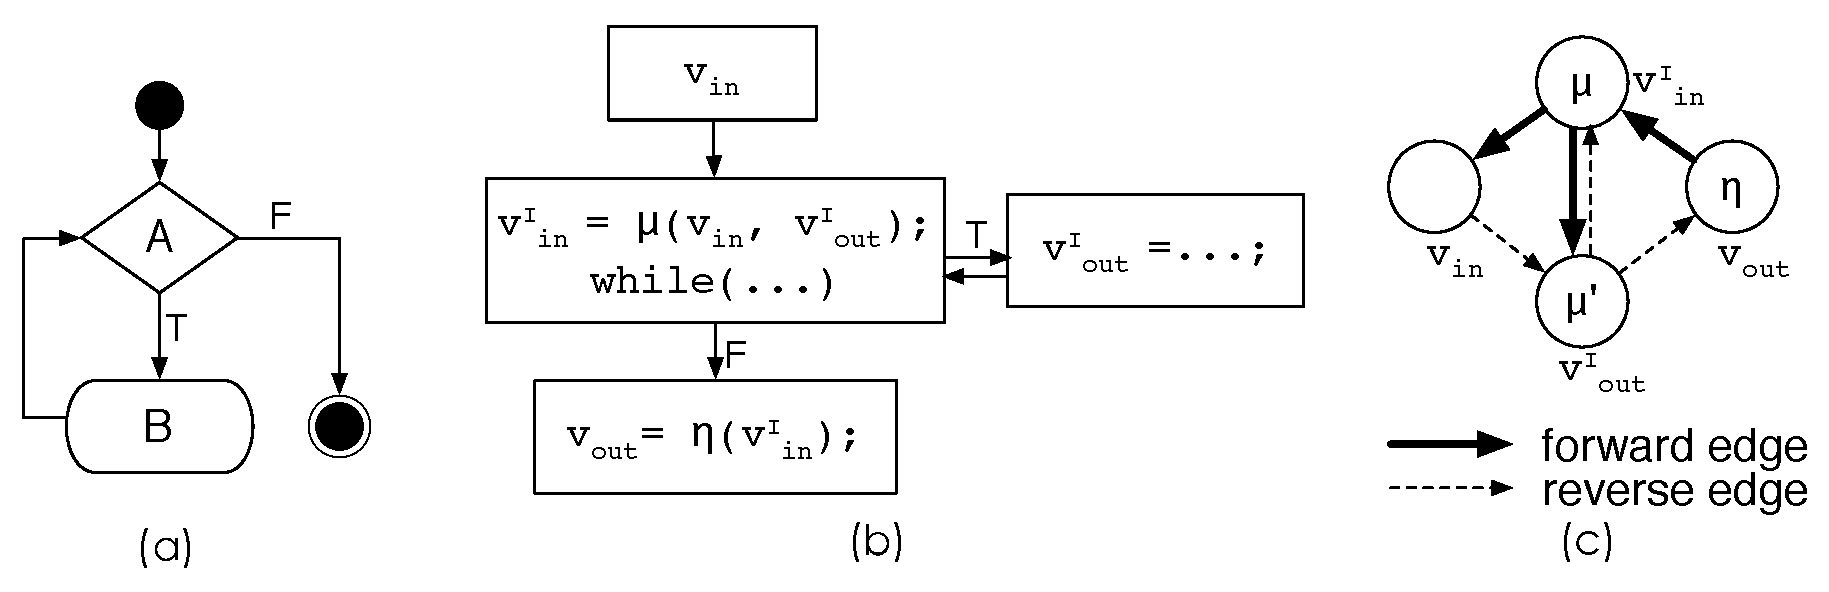
\includegraphics[width=400pt]{figures2/simpleLoop.pdf}}
\caption{(a) The diagram of a while loop. (b) The CFG in loop-closed SSA form for a variable $v$ modified in the loop. (c) Forward and reverse edges.}
\label{fig:loop_example}
\end{figure}

\subsection{Dealing with while loops}
\label{sec:while-loops}

%Let's first look at a simple while loop example. 
We first consider a while loop with the diagram shown in Figure~\ref{fig:loop_example}(a).
We further assume that $A$ has no side-effects %
%
%\footnote{A more loose condition is that a definition can exist in $A$ as long as this definition is only ``live'' in the loop, i.e., is not used outside of the loop.}
%
and that there are no escapes from $B$.
Thus, the loop only exits from its entry.  

Given such a while loop, we transform it into the \emph{loop-closed SSA form}~\cite{Pop2009}, illustrated in Figure~\ref{fig:loop_example}(b).
Loop-closed SSA differs from conventional loop-free SSA as follows.
In conventional SSA, a special marker called a \emph{$\phi$ function} is placed in the CFG at the first program point where two distinct versions (definitions) of a variable, computed along different program paths, meet.
%
In loop-closed SSA, if a value is defined inside of a loop and used outside of it, we place a special single entry $\phi$ function at the \emph{exit} of the loop.
To distinguish this type of loop-specific $\phi$ function from a conventional $\phi$ function as used in loop-free programs, we denote the loop-specific form by the term $\eta$ function, by convention~\cite{RobertA.Ballance1990}.
Additionally, suppose a definition of a variable from outside the loop and a definition coming from a back-edge of the loop meet at a program point.
Again, we create a $\phi$ function marker here, and to distinguish it, we refer to it as a $\mu$ function.

To see how these markers work, consider a variable $v$ modified by a while loop;
we now describe the corresponding loop-closed SSA form, which Figure~\ref{fig:loop_example}(b) illustrates.
Let \vinit denote the input value of $v$ before the loop executes, and \vfinal the output value of $v$ after the loop executes.
Next, let the input to the loop \emph{body} be \vmu and the output \viter.
(The superscript $I$ is intended to remind the reader that these are values associated with an \emph{iteration} of the loop, as opposed to the values before and after the loop.)
Then, \vmu is defined by a $\mu$ function as \mufunc, and \vfinal is defined by a $\eta$ function as \etafunc.
That is, \mufunc indicates the program point at which $v$ has either the initial value before the loop executes or the value produced by some iteration of the loop;
and \etafunc indicates the program point at which $v$ has the final value once the loop completes.
%We will consider the problem how to generate a forward loop 
%Now let's construct the VSG for generating the forward and reverse loops.

From this loop-closed SSA form, we wish to build a VSG that will express equality relations among the four SSA values, \vinit, \vfinal, \vmu, and \viter.
This VSG result is shown in Figure~\ref{fig:loop_example}(c).
Recall that nodes in the VSG represent values, and edges the equality relations.
%
%The loop-collapsed \pVSG comes from the left-hand column of nodes from Figure~\ref{fig:loop_example}(b) and is shown in Figure~\ref{fig:loop_example}(c) as the upper three nodes and upper two solid edges.
%The loop body \lVSG comes from the right-hand node of Figure~\ref{fig:loop_example}(b) and results in the bottom node of Figure~\ref{fig:loop_example}(c).
%
%Now we consider the problem how to retrieve \vfinal or \vinit from \lVSG.
%If we could do that, a loop will be generated in the reverse program producing \vfinal or \vinit.
%
There are four value nodes.
The nodes \vinit and \vfinal are part of the loop-collapsed \pVSG, and \vmu and \viter belong to the loop body's \lVSG.
The $\mu$ and $\eta$ functions indicate how to connect \pVSG and \lVSG.
In particular, the three solid bold edges are associated with the dependences induced by executing the loop in the forward direction;
we call these the \emph{forward edges}, and a $\mu$ node is incident to all three.
The presence of these edges make it possible to obtain \vfinal by some path passing through \lVSG, and simultaneously indicate that a loop is present for subsequent code generation.
Similarly, the three dashed edges are \emph{reverse edges} associated with dependences induced in the reverse direction.
These edges make it possible to obtain \vinit by some path through \lVSG.
Note that the reverse edges form a symmetry to the forward edges.
From this symmetry, we define the node incident to all three reverse edges as a $\mu'$ node.
Later we will show how the search traverses these edges.

Having built the CFG, the next step is to search it, producing the RG result.
Recall from Section~\ref{sec:backstroke} that we are given a set of target nodes whose values we wish to eventually compute from a starting set of available nodes.
We search for a path from available nodes to target nodes; the subgraph representing paths is the RG, which is not necessarily unique.
Our algorithm is similar to the one we have described previously~\cite{Hou2012}, but for loops we need three additional search rules:

\begin{itemize}
\item During a search for a value, once a forward/reverse edge is selected, all edges in the other category cannot be chosen. This is because either a forward or a reverse loop will be built to retrieve the value.

%To build a forward loop, if the search reaches a $\mu$ node, it forks by advancing through the two outgoing forward edges; to build a reverse loop, if the search reaches a $\mu'$ node, it forks by advancing through the two outgoing reverse edges. 
\item When the search reaches a $\mu$ or $\mu'$ node, it will be split into two sub-searches, in \pVSG and \lVSG, respectively, through the two outgoing forward or reverse edges.
For example, in Figure~\ref{fig:loop_example}(c), if the search reaches \vmu, the algorithm begins two sub-searches beginning with \vinit and \viter.

%As we discussed above, if at compile time we can determine that the loop body will certainly be traversed at runtime, the search does not fork but continues toward \viter or \vmu.
\item During the search, the algorithm may form a directed cycle only in \lVSG; furthermore, such a cycle must contain a forward or reverse edge between a $\mu$ and $\mu'$ node. 
Once a cycle is formed, the search in \lVSG is complete.
%will not move further from the current node just like when an available node is reached.
\end{itemize}

\noindent
We build a while loop as either a forward or a reverse loop. 
Synthesizing such a while loop consists of synthesizing its body and predicate.


\subsubsection{Building the loop body.}

The loop body in the reverse program is generated from the search result in \lVSG.
For each variable we remove the edge between the $\mu$ and $\mu'$ nodes and hence remove the cycles, so that we can generate the loop body using our prior code generation algorithm~\cite{Hou2012}.

%there is no cycles any more. 
%As a result, this subgraph of the RG used to build the loop body connects each \viter or \vmu (for forward or reverse loop) to the $\mu$/$\mu'$ node or value nodes not defined in the loop. The code is generated in the same method as in \cite{Hou2012}. 
%Since recording control flows in a loop may be expensive, we will use the method mentioned in the previous section which retrieves each value in the predicate. If this method does not work, we have to record the control flows for all iterations using a bit vector. It is possible that the cost to store control flows offsets the benefit to retrieve a value from a loop which may not need a state saving. In this case, we can turn to the method in \cite{Hou2012} which is a better choice.

\begin{comment}

\begin{figure}%[htb]
\center{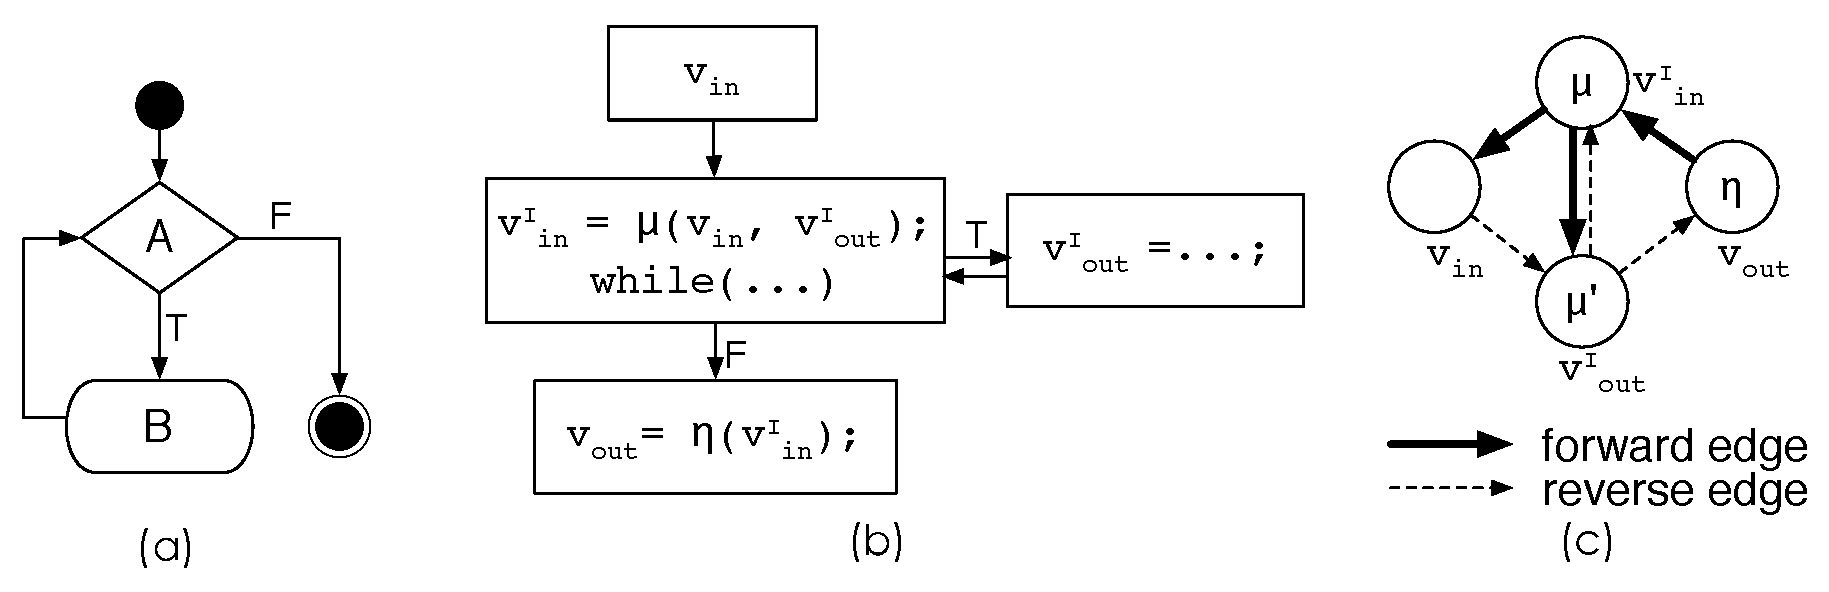
\includegraphics[width=300pt]{figures2/loopExample.pdf}}
\caption{(a) The VSG for our example. (b) The RG for retrieving $a_3$ and $i_3$. (c) The RG for retrieving $a_0$.}
\label{fig:loopExample}
\end{figure}

\end{comment}



%Our search begins from the node $a_0$ in Figure \ref{fig:loop_vsg}(a). Once we go from $a_0$ to $a_1$ into the loop block\footnote{\TODO{need we define this term?}}, we are selecting to build a reverse loop, and we will add some restrictions during the search: all edges belonging to the forward execution should not be taken. 

%In [], we forbid any circle during the search for each CFG path, however, since we are building another loop, we permit the circle to appear in the search result, with one requirement: each circle should contain the edge between $v_{\mu}$ and $v_{iter}$.



%The loop body generated from Figure \ref{fig:loop_vsg}(b) is \texttt{\{ i = i + 1; a = a + i;  \}}, and the loop body generated from Figure \ref{fig:loop_vsg}(c) is \texttt{\{ a = a - i;  i = i - 1; \}}.


\subsubsection{Building the loop predicate.}

To guarantee that the generated loop has the same iterations at runtime as the original loop, we need to build a proper loop predicate. 
We propose three approaches to building a correct loop predicate. 
To illustrate those approaches, we temporarily introduce the following loop example. We assume that the omitted statements  modify neither \texttt{A[]} nor \texttt{i}.


\small
\begin{verbatim}
                              i = 0;
                              while (A[i] > 0) {
                                  /* ... */
                                  i = i + 2;
                              }
\end{verbatim}
\normalsize


%The first two approaches are preferred since they may not need any instrumentation to the original loop, but cannot be always applied, and the third one needs an instrumentation to the forward program and is always working. 

\begin{itemize}
\setlength{\itemsep}{5pt}%

\item \textbf{Approach 1:} Building the same loop predicate as that in the original loop. 
To build this predicate, we need to retrieve each value in the predicate.
%, we need to retrieve its input value of the loop before the loop, and if it is updated in the loop, we also need to retrieve its input value of the loop body in the loop. 
A new search is needed to acquire those values, and the search result will be combined into the RG generated above.
For the example above, we can build a loop below that has the same number of iterations as the original one. The omitted statements will be substituted by the loop body built above.



\small
\begin{verbatim}
                          i = 0;
                          while (A[i] > 0) {
                              /* ... */
                              i = i + 2;
                          }
\end{verbatim}
\normalsize


%In the second case, we  
%$a$ for example, if it is not modified in the loop, we need to retrieve the value of $a$ before building the while condition; if it is defined by a $\mu$ function as $a_{in}^I = \mu (a_{in}, a_{out}^I)$, both $a_{in}$ and $a_{out}^I$ should be retrieved. 
%Figure \ref{fig:rvsLoops}(a) shows the resulted loop built from this approach.
%This is done by starting another search beginning with $a_{in}^I $. Note that we also updated the loop body to include the statement that defines $a_{out}^I$.


\item \textbf{Approach 2:} Building the loop predicate from a variable updated in the loop. Given a variable $v$ and its four definitions: \vinit, \vmu, \viter, and \vfinal, if \vmu$\ne$\vfinal in each iteration except the last definition of \vmu (which is actually \vfinal), and if we can retrieve \vinit and \vfinal before the loop (hence we cannot retrieve them through the loop), and \viter in the loop, we can use them to build a while loop as:
$$
u := v_{in}; \; while (u \ne v_{out}) \;  \{\; /* \; update \; u \; */ \; \}
$$

Similarly, if \viter$\ne$\vinit  in each iteration, and  \vinit and \vfinal can be retrieved before the loop, and \vmu can be retrieved in the loop, we can use them to build a while loop as: 

$$
u := v_{out}; \; while (u \ne v_{in}) \;  \{\; /* \; update \; u \; */ \; \}
$$

In general, it is difficult to detect all variables satisfying the properties above.
However, there are some special cases.
One case is that of \emph{monotonic variables}~\cite{Wolfe1992}, which are monotonically strictly increasing or decreasing in each iteration.
Another is that of induction variables, which are special monotonic variables that are relatively easier to recognize. In the above example, \texttt{i} is an induction variable. Assume its final value after the loop is \texttt{i1} that is known, and then we can build the following loop with the predicate using \texttt{i}.



\small
\begin{verbatim}
                          i = 0;
                          while (i != i1) {
                              /* ... */
                              i = i + 2;
                          }
\end{verbatim}
\normalsize


%Indeed, the first approach above is a special case of this one if we define another Boolean variable $c$ as $a < b$, where $c$ satisfies the condition above.
 %Instead, we only detect variables which are updated during iterations monotonically. Note that induction variables fall into this category which are easier to detect.
%loop variant. A loop variant is a variable whose value is updated in each iteration monotonically\footnote{This is too strict: \TODO{distinct values are also OK.}} and the while condition is a comparison between the loop variant and another value. Assume the loop variant is $i$ with initial value $i_{init}$ and final value $i_{final}$, and in all iterations, $i$ is increased or decreased monotonically. If we can retrieve $i_{init}$ and $i_{final}$, plus $i_{\mu}$ or $i_{iter}$ in each iteration, we can use this variable to build the while condition for the forward or reverse loop. Specifically, a forward loop \TODO{Note that it does not make sense to classify a loop as a forward or reverse one, since they may appear in the same loop} is built like:
%To build the while condition, we first detect all loop variants in the loop (\TODO{how?}). For each loop variant $i$, we have to retrieve both $i_{init}$ and $i_{final}$, and depending on whether the generated loop is forward or reverse, we have also to retrieve either $i_{\mu}$ or $i_{iter}$. 
%Because at the beginning of the loop, we should already have $i_{init}$ and $i_{final}$, we cannot retrieve them through the loop. This means the search should not reach the loop nodes from them. The search for $i_{\mu}$ or $i_{iter}$ follows two forward or reverse edges as described above. 
%In case that there are several candidates satisfying the requirement above, for each variable, we calculate the cost to retrieve all dependent values and choose one with the least cost to build the loop predicate. 
%In our example, both $a$ and $i$ are monotonic variables, but  $a$'s initial value is unknown (which is what we are retrieving!). In contrast, $i$'s initial and final value are 0 and $N$, and $i$ can be updated either by a forward loop beginning with its initial value, or a reverse loop beginning with its final value. Figure \ref{fig:rvsLoops}(b) and (c) shows those two results. Note that in Figure \ref{fig:rvsLoops}(c) the code retrieving $i$ in the loop body is shared with the loop body generated before \TODO{!}.


\begin{comment}
\begin{figure}%[htb]
\center{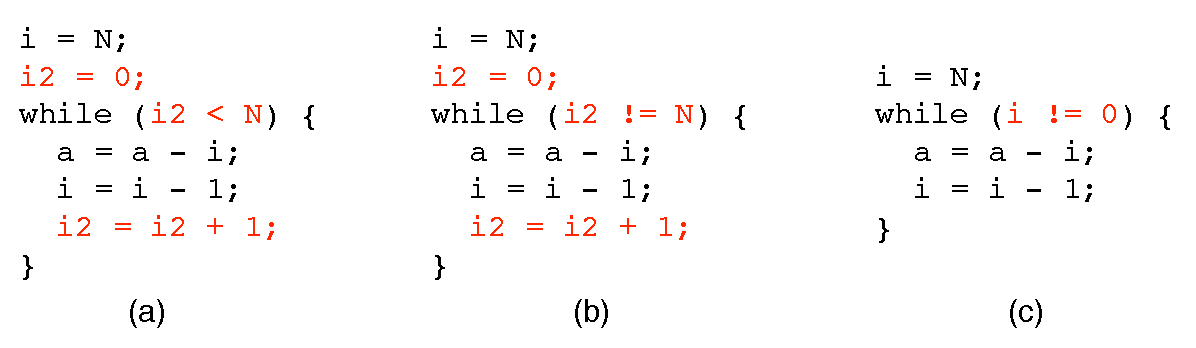
\includegraphics[width=300pt]{figures2/reverseLoops.pdf}}
\caption{Three results.}
\label{fig:rvsLoops}
\end{figure}
\end{comment}

%However, it is possible that we cannot find such a loop variant. (Although every loop that terminates has a variant). 
%The reason is that the loop variant we are looking for is somehow special, but it is possible \TODO{see wiki: Transfinite induction}. 
\item \textbf{Approach 3:} Instrumenting the original loop with a counter counting the number of iterations. The counter has the initial value zero and is incremented by one on each back edge of the loop.
The final value of the counter is stored in the forward program and restored in the reverse program as the maximum value of another loop counter.
This approach generally works if either of the above two approaches fail.
However, it requires instrumentation (the counter), and therefore forces generation of a forward program. Below we show the instrumented loop in the forward program (left) and the generated loop in the reverse program (right) for the above example.


\small
\begin{verbatim}
        i = count = 0;                   restore(count);
        while (A[i] > 0) {               while (count > 0) {
            /* ... */                        /* ... */
            i = i + 2;                       count = count - 1;
            count = count + 1;           }
        }                             
        store(count);
\end{verbatim}
\normalsize



\end{itemize}

We prioritize these approaches as follows.
Applicability and state-saving cost are our main criteria.
We prefer Approach 1 and 2 over 3.
When either 1 or 2 apply, if no state-saving is required, we apply them.
Otherwise, we try Approach 3 and choose the overall approach with the least cost.

\vspace{3mm}

\begin{figure}%[htb]
\center{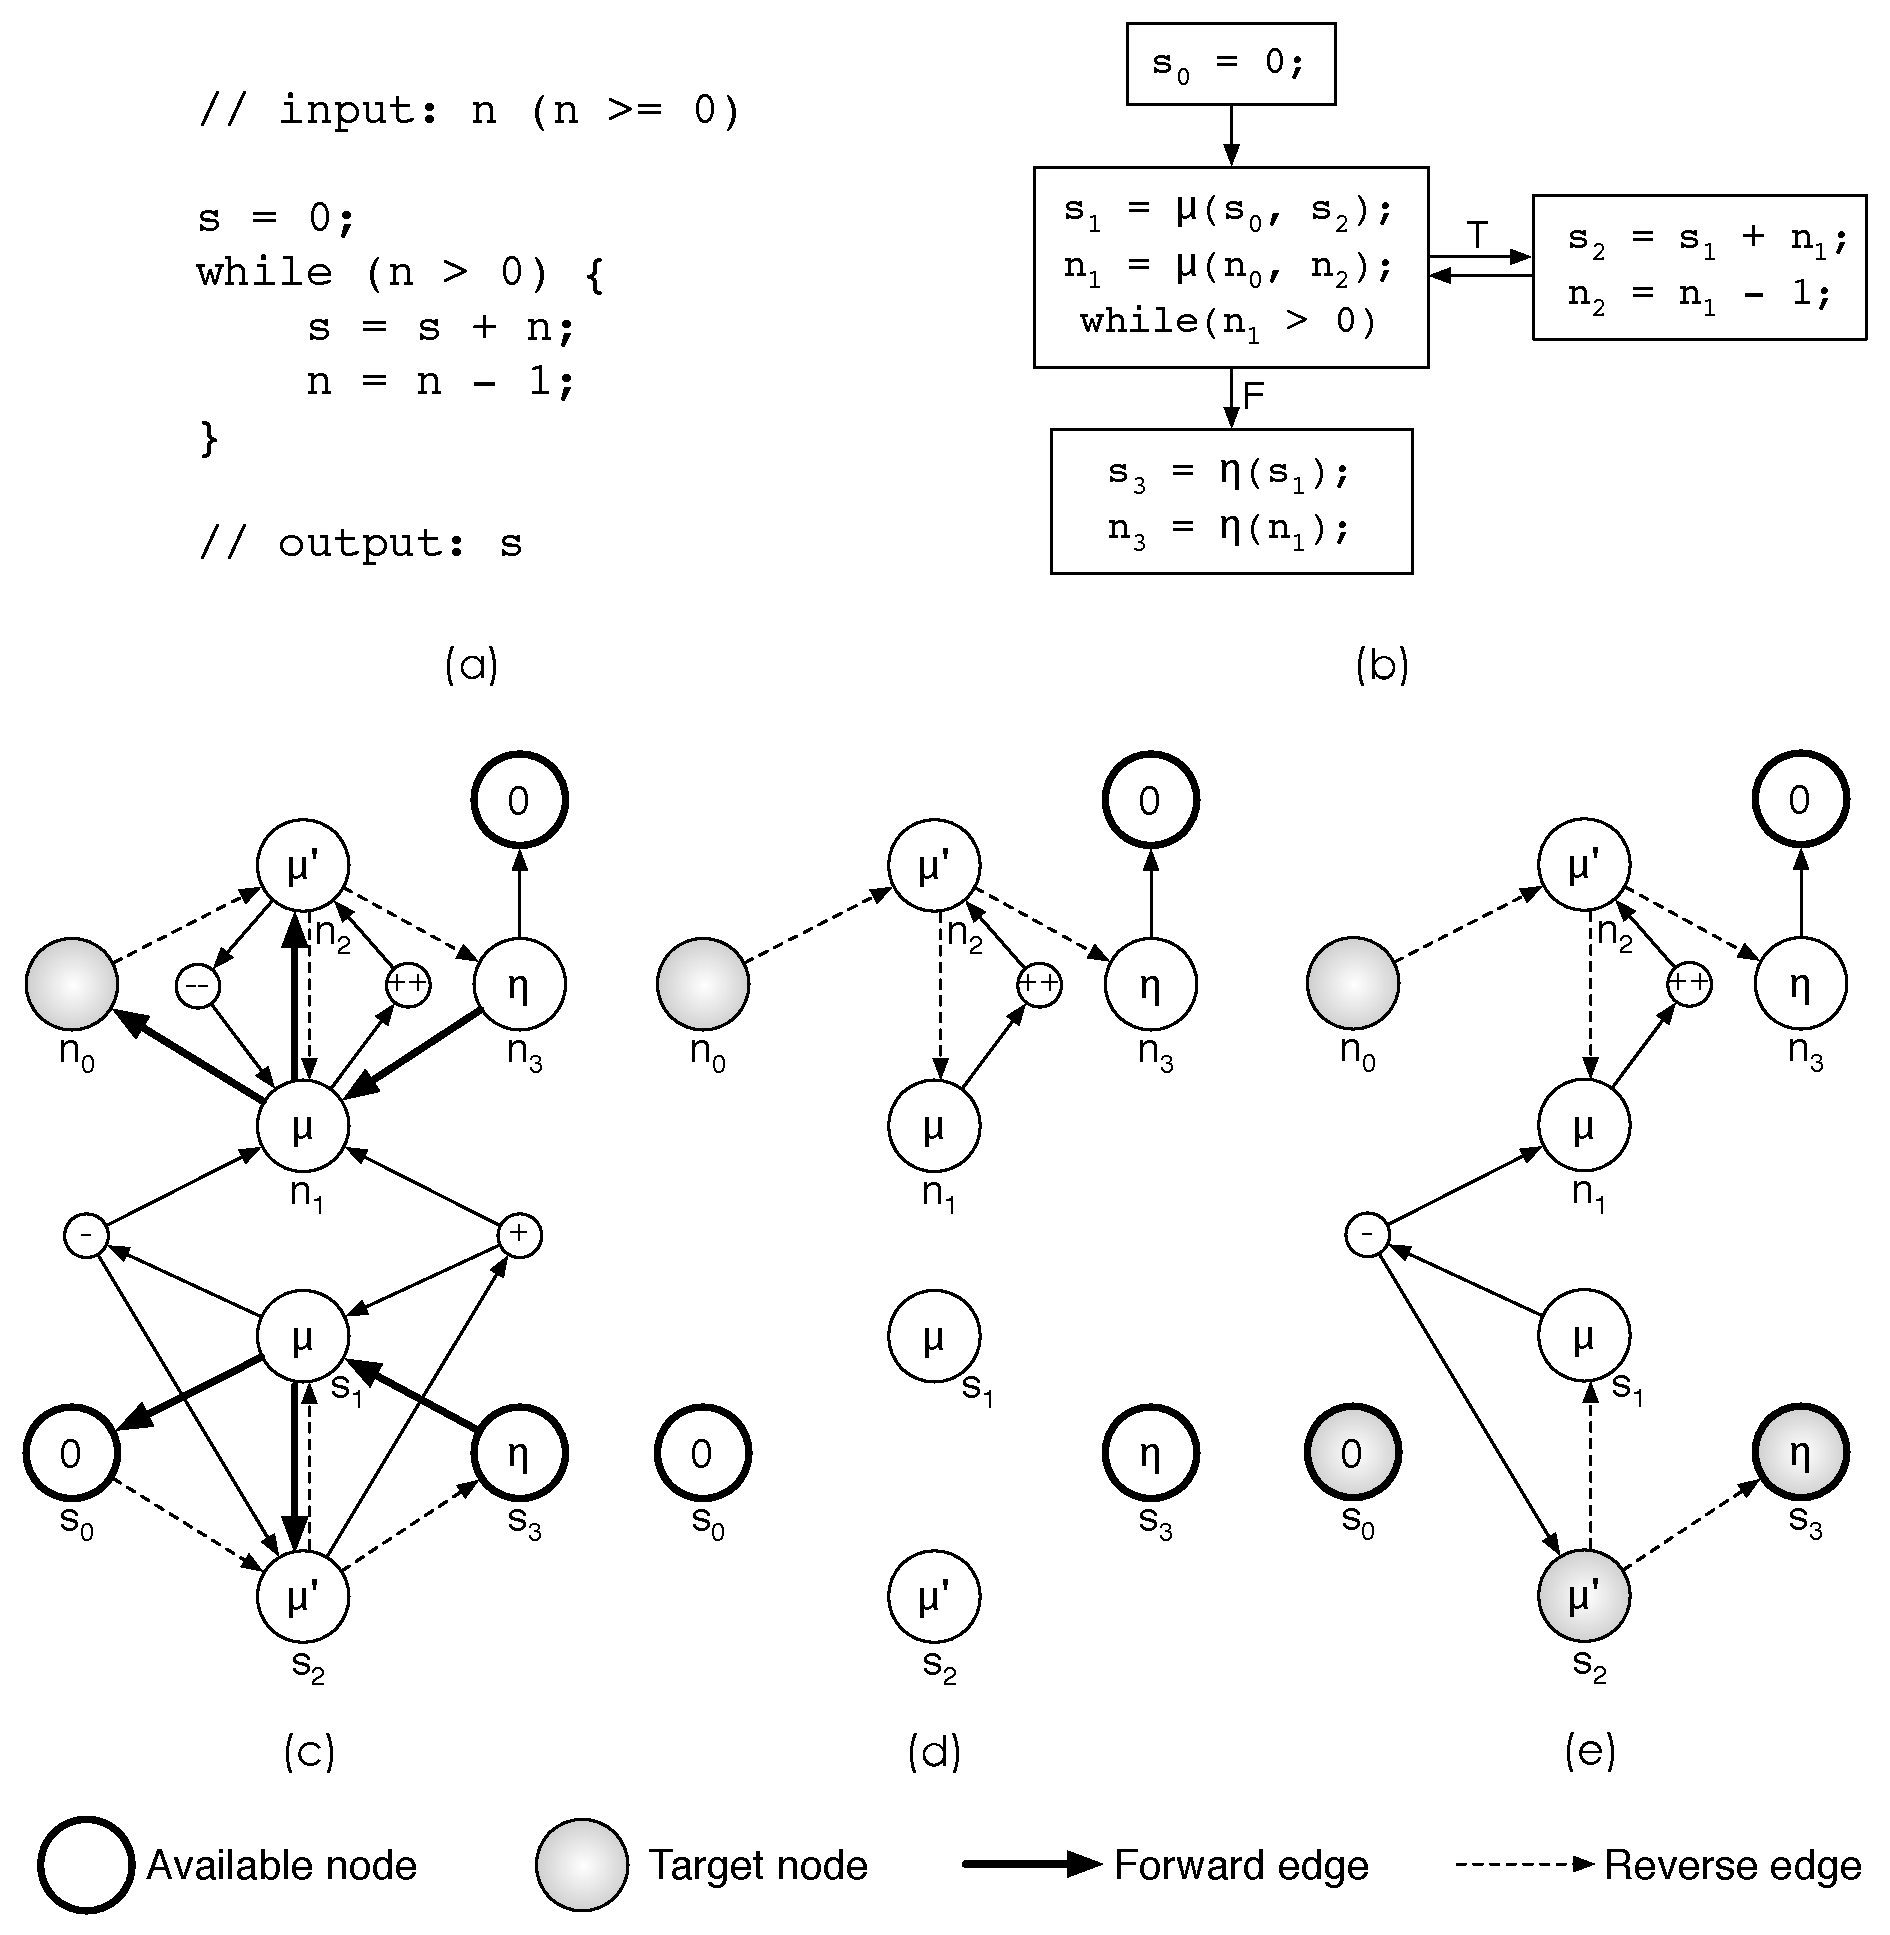
\includegraphics[width=400pt]{figures2/loopVSG.pdf}}
\caption{(a) The program of our example. (b) The CFG in loop-closed SSA form. (c) The VSG.  (d) The RG for retrieving $n_3$. (e) The RG for retrieving $n_0$ and $s_2$.}
\label{fig:loop_vsg}
\end{figure}

As an example, suppose we apply this algorithm to the loop in Figure~\ref{fig:loop_vsg}(a).
Figure \ref{fig:loop_vsg}(b) shows its CFG in loop-closed SSA.
The input is $n_0$ and the output $s_3$.
Our goal is to generate a reverse program that takes $s_3$ as input and produces $n_0$.
We build the VSG shown in Figure~\ref{fig:loop_vsg}(c), with forward and reverse edges shown as bold and dashed edges, respectively.
Note that the equality between $n_3$ and 0 is acquired from solving constraints, a standard compiler technique, as discussed in Section~\ref{sec:discussions}.%
%
\footnote{For clarify, we remove the equality $n_1=s_2-s_1$, as this relation will not be used during the search.}
%
The search result for value $n_0$ is shown in Figure \ref{fig:loop_vsg}(d), from which we can build the loop body as \texttt{\{ n = n + 1;  \}}.

Next, we build the loop predicate.
In our example, because we wish to retrieve the initial value of $n$, we cannot use it to build the loop predicate.
We can discover that $s$ is a monotonic variable, and that both the initial and final values of $s$, which are 0 and $s_3$, respectively, are available.
To get $s_2$, we search its value on the VSG and the search result is shown in Figure \ref{fig:loop_vsg}(e). 
As a result, we build the loop predicate from $s$ and the reverse program is generated as below.

\small
\begin{verbatim}
                              n = 0;
                              while (s != 0) {
                                  n = n + 1;
                                  s = s - n;
                              }
\end{verbatim}
\normalsize


\begin{comment}

Above we have built a reverse loop in the reverse program, but it is also possible that the reverse program contains a forward loop. 
For instance, if we change our example into the program shown  below left, without modifying its semantic, its inverse will contain a forward loop which is shown on the right. This is because the input of the new program $n_0$ is equal to $i$'s final value, which is the output of the loop. 
\begin{verbatim}
          s = 0;                     s2 = 0; 
          i = 0;                     i = 0;
          while (i < n) {            while (s2 != s) {
            i = i + 1;                 i = i + 1;
            s = s + i;                 s2 = s2 + i;
          }                          }
                                     n = i;
\end{verbatim}

\end{comment}

%\subsubsection{Other single-exit loops}
%The while loop we discussed above is just one kind of the single-exit loops. %Do-while loop is another single-exit loop. 
%For other single-exit loops, we can transform them into while loops, and we can also utilize the similar technique as above to handle them. However, as we will see later, the transformation described below can handle those cases including loops with several exits. 

\subsection{Dealing with loops other than while loops}
\label{sec:other-loops}

In practice, the vast majority of loops have a single entry, which are called \emph{natural loops}~\cite{Muchnick}. 
Loops with more than one entry are quite rare and can in fact be transformed into natural loops~\cite{Muchnick}. 
However, it is quite common that a loop has several exits. 
For example, in C/C++ we may exit a loop early through \texttt{break}, \texttt{return}, or \texttt{goto} statements.
Nevertheless, given a non-while natural loop, we can transform it to separate the last iteration from the loop;
then, the remaining iterations form a new while loop, and the last iteration will not belong to the loop and hence can considered with the control flows outside of the loop. 
We then process the new while loop as previously described.
Note that this ``transformation'' is only applied to the CFG during the analysis, and not to the original program.
As such, in the forward program \Forward the last iteration and other iterations of each loop continue to share the same code.


Figure~\ref{fig:loop}(a) shows a loop in a CFG, with a header (node 1) and two back edges (4$\to$1 and 5$\to$1). 
There are two different exits from this loop, which are nodes 6 and 7.
%An exit edge of a loop is an edge connecting a loop node to an exit. 
%1$\to$6 and 3$\to$7 are two exit edges.
Figure~\ref{fig:loop}(b) shows the CFG of the transformed loop.
This transformation is performed as follows.

In a natural loop, only the last iteration takes the exit, and any other iteration goes back to the loop header.
Therefore, if the last iteration is peeled off from the loop, this loop will turn into a while loop. 
%Suppose we can predicate the number of iterations (the number of back edges being traversed) before a loop is taken, which is although impossible for most loops. Let \texttt{k}  be a virtual variable whose value is the number of the back edges being taken at runtime, 
To implement this transformation, we create a new branch node with an unknown predicate that returns $true$ if the next iteration is not the last one and $false$ otherwise.
Note that we will not build this predicate in the forward program. 
The new branch node turns over all in-edges of the loop header. 
%Note that  \texttt{k}'s initial value usually cannot be determined at compile time, but we are not actually doing this transformation to the original function and hence it won't bring any problem here. 
Its $true$ labeled out-edge will point to the loop header of a copy of the loop (node $1'$) with back edges but without exit edges, and all back edges are redirected to this new branch node making it a new loop header. 
Note that after removing exit edges it is possible that a previous branch node becomes a non-branch node (node $3'$, for example), which is fine because the removed branch edge will not be taken. Then, we can remove the (side effect free) predicates from those nodes. The edge labeled with $false$ from the new branch node will point to the original loop header (node 1) and all back edges in the original loop are removed, since the last iteration won't take the back edge. The nodes from which the exit of the program is not reachable due to the back edge removal are removed (node 4 and 5, for example). Again the predicate is removed from a node once it is not a branch node anymore (node 2 and 3).
%Fig \ref{fig:loop}(b) shows the transformed flow graph where the node 0 is the new branch node and loop header. Note that the node 4 and 5 are removed since they are not reachable anymore.
 %At runtime, the true edge must be traversed and the false edge may not. 
%The true edge postdominates the false edge, but the latter does not dominate the former. 

\begin{figure}%[htb]
\center{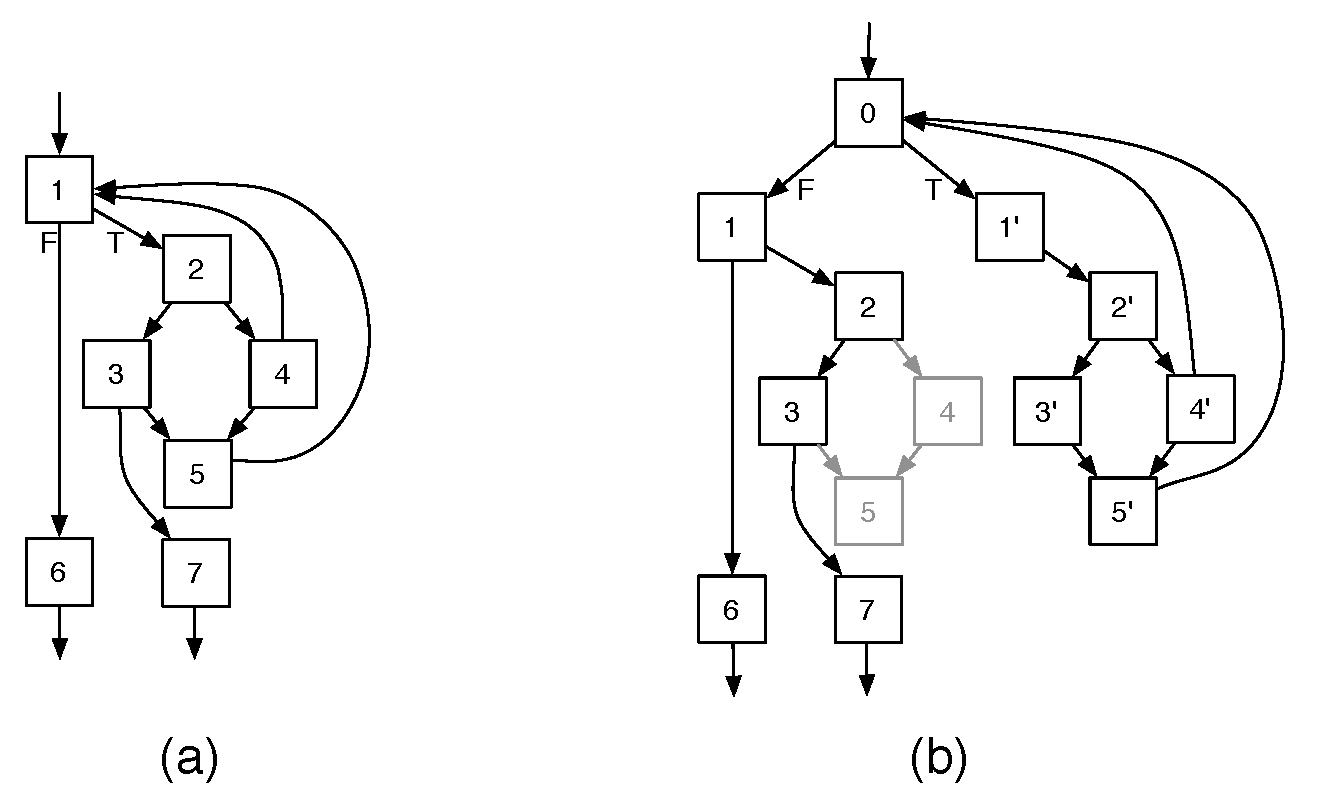
\includegraphics[width=350pt]{figures2/Loop.pdf}}
\caption{(a) A loop in CFG with two back edges and two exits. (b) The CFG of the transformed loop.}
\label{fig:loop}
\end{figure}

After the transformation, all loops in the program become while loops and our method applies.
%Since the new generated loop predicate  is unknown, to build the predicate of the loop in the reverse program, we cannot use the first approach proposed above any more. Therefore, it is preferred that a loop be transformed into a while loop normally, not in the above method. For example, a do-while loop can be easily converted into a while loop.

%Because the new loop and the epilog share the same code in the forward function,  any instrumentation will also be shared between them. For example, if a value defined in the epilog needs a state saving, we can only perform the state saving in the loop, which results in saving a value many times and then time overhead. Properly defining the cost of this operation may help to get the better search result. % On the other hand, if a state saving is made from reversing the loop hammock, at the exit of the loop, any side effect should be taken care. For example, if a stack is used to store variables, the pop operations may be needed at the exits.






\chapter{Synthesis for programs with arrays}

\chapter{Conclusion}

\nocite{*}
%% We need this since this file doesn't ACTUALLY \cite anything...
%%
\appendix
\chapter{Some Ancillary Stuff}

Ancillary material should be put in appendices, which 
appear just before the bibliography. 

\begin{postliminary}
\references


\end{postliminary}

\begin{abstract}
  This is the abstract that must be turned in as hard copy to the
  thesis office to meet the UMI requirements. It should \emph{not} be
  included when submitting your ETD. Comment out the abstract
  environment before submitting. It is recommended that you simply
  copy and paste the text you put in the summary environment into this
  environment. The title, your name, the page count, and your
  advisor's name will all be generated automatically.
\end{abstract}

\end{document}
